% Options for packages loaded elsewhere
\PassOptionsToPackage{unicode}{hyperref}
\PassOptionsToPackage{hyphens}{url}
%
\documentclass[
]{article}
\usepackage{lmodern}
\usepackage{amssymb,amsmath}
\usepackage{ifxetex,ifluatex}
\ifnum 0\ifxetex 1\fi\ifluatex 1\fi=0 % if pdftex
  \usepackage[T1]{fontenc}
  \usepackage[utf8]{inputenc}
  \usepackage{textcomp} % provide euro and other symbols
\else % if luatex or xetex
  \usepackage{unicode-math}
  \defaultfontfeatures{Scale=MatchLowercase}
  \defaultfontfeatures[\rmfamily]{Ligatures=TeX,Scale=1}
\fi
% Use upquote if available, for straight quotes in verbatim environments
\IfFileExists{upquote.sty}{\usepackage{upquote}}{}
\IfFileExists{microtype.sty}{% use microtype if available
  \usepackage[]{microtype}
  \UseMicrotypeSet[protrusion]{basicmath} % disable protrusion for tt fonts
}{}
\makeatletter
\@ifundefined{KOMAClassName}{% if non-KOMA class
  \IfFileExists{parskip.sty}{%
    \usepackage{parskip}
  }{% else
    \setlength{\parindent}{0pt}
    \setlength{\parskip}{6pt plus 2pt minus 1pt}}
}{% if KOMA class
  \KOMAoptions{parskip=half}}
\makeatother
\usepackage{xcolor}
\IfFileExists{xurl.sty}{\usepackage{xurl}}{} % add URL line breaks if available
\IfFileExists{bookmark.sty}{\usepackage{bookmark}}{\usepackage{hyperref}}
\hypersetup{
  pdftitle={Reassessing the Role of Theory and Machine Learning in Forecasting Civil Conflict},
  pdfauthor={Andreas Beger; Richard K. Morgan; Michael D. Ward},
  hidelinks,
  pdfcreator={LaTeX via pandoc}}
\urlstyle{same} % disable monospaced font for URLs
\usepackage[margin=1in]{geometry}
\usepackage{longtable,booktabs}
% Correct order of tables after \paragraph or \subparagraph
\usepackage{etoolbox}
\makeatletter
\patchcmd\longtable{\par}{\if@noskipsec\mbox{}\fi\par}{}{}
\makeatother
% Allow footnotes in longtable head/foot
\IfFileExists{footnotehyper.sty}{\usepackage{footnotehyper}}{\usepackage{footnote}}
\makesavenoteenv{longtable}
\usepackage{graphicx}
\makeatletter
\def\maxwidth{\ifdim\Gin@nat@width>\linewidth\linewidth\else\Gin@nat@width\fi}
\def\maxheight{\ifdim\Gin@nat@height>\textheight\textheight\else\Gin@nat@height\fi}
\makeatother
% Scale images if necessary, so that they will not overflow the page
% margins by default, and it is still possible to overwrite the defaults
% using explicit options in \includegraphics[width, height, ...]{}
\setkeys{Gin}{width=\maxwidth,height=\maxheight,keepaspectratio}
% Set default figure placement to htbp
\makeatletter
\def\fps@figure{htbp}
\makeatother
\setlength{\emergencystretch}{3em} % prevent overfull lines
\providecommand{\tightlist}{%
  \setlength{\itemsep}{0pt}\setlength{\parskip}{0pt}}
\setcounter{secnumdepth}{5}
\usepackage{floatrow}
\floatsetup[figure]{capposition=bottom}
\floatsetup[table]{capposition=top}
\usepackage[format=plain,labelfont=bf,up]{caption}
\usepackage{setspace}\doublespacing
\usepackage{booktabs}
\usepackage{longtable}
\usepackage{array}
\usepackage{multirow}
\usepackage{wrapfig}
\usepackage{float}
\usepackage{colortbl}
\usepackage{pdflscape}
\usepackage{tabu}
\usepackage{threeparttable}
\usepackage{threeparttablex}
\usepackage[normalem]{ulem}
\usepackage{makecell}
\newlength{\cslhangindent}
\setlength{\cslhangindent}{1.5em}
\newenvironment{cslreferences}%
  {\setlength{\parindent}{0pt}%
  \everypar{\setlength{\hangindent}{\cslhangindent}}\ignorespaces}%
  {\par}

\title{Reassessing the Role of Theory and Machine Learning in Forecasting Civil Conflict\thanks{John Ahlquist, Cassy L. Dorff, and Shahryar Minhas both provided helpful feedback on this project. We are especially grateful to Paul Huth for his comments and guidance. All the code and several additional analyses can be found at our replication archive at \url{https://github.com/andybega/Blair-Sambanis-replication}.}}
\author{Andreas Beger\footnote{Predictive Heuristics, \href{mailto:adbeger@gmail.com}{\nolinkurl{adbeger@gmail.com}}.} \and Richard K. Morgan\footnote{Independent Researcher, \href{mailto:rick.morgan2@gmail.com}{\nolinkurl{rick.morgan2@gmail.com}}.} \and Michael D. Ward\footnote{Predictive Heuristics, Duke University, University of Washington, \href{mailto:michael.don.ward@gmail.com}{\nolinkurl{michael.don.ward@gmail.com}}. Corresponding author.}}
\date{12 November 2020}

\begin{document}
\maketitle
\begin{abstract}
We examine the research protocols in Blair and Sambanis (nd), who argue that their theory-based model can predict civil war onsets better than several atheoretical alternatives or a model with country-structural factors. We find that there are several important mistakes and that their key finding is entirely conditional on the use of parametrically smoothed ROC curves when calculating accuracy, rather than the standard empirical ROC curves that dominate the literature. Fixing these mistakes results in a reversal of their claim that theory-based models of escalation are better at predicting onsets of civil war than other kinds of models. Their model is outperformed by several of the ad hoc, putatively non-theoretical models they devise and examine. More importantly, we argue that rather than trying to contrast the roles of theory and "atheoretical" machine learning in predictive modeling, it would be more productive to focus on ways in which predictive modeling and machine learning could be used to strengthen extant predictive work. Instead, we argue that predictive modeling and machine learning are effective tools for theory testing.
\end{abstract}

\hypertarget{introduction}{%
\section{Introduction}\label{introduction}}

Blair and Sambanis (n.d., hereafter B\&S) argue that theory is essential for creating models that have high accuracy in forecasting civil war onset. Indeed, they assert that with such theory forecasting is more accurate than has previously been possible. We re-examine the empirical basis for the claims made in support of it. We find that these claims to be unsupported and evidence presented for them to be incorrect. Their theory-based escalation model does not do better than the alternatives they examine. It does worse. The reason for this is that they made several mistakes in their research procedure. Further, the performance results they report are based on smoothed performance curves, not the empirical, unsmoothed curves. This provides misleading results. In addition, two of the structural alternatives to their basic escalation model were incorrectly implemented. We also found that the scoring of their forecasts for the first half of 2016 was incorrectly performed using civil war incidence, not onset. In what follows, we show the impact of these mistakes on the conclusions.

B\&S claim (page 3) to argue that a model informed by procedural theories of escalation and de-escalation can predict the onset of civil wars ``remarkably accurately''. Indeed, B\&S argue that this theoretical model outperforms four other ``more mechanical'' alternatives. They also claim that the integration of structure with process is better than alternatives over short forecasting windows. Third, they preregistered the list of thirty countries that have the highest risk of civil war onset. They claim that such prospective predictions are rare in the literature when, in fact, they have been routine for many years with several prominent projects.\footnote{PITF (e.g., Goldstone et al. 2010; Beger and Ward 2017), the W-ICEWS project (Ward et al. 2013), ViEWS (Hegre et al. 2019), and others, e.g., Beger, Morgan, and Maxwell (2020).} B\&S claim to be unique in assessing these forecasts. A qualitative analysis of their predictions allows them to conclude that their model is robust. We will return to their analysis later, after correcting the procedural mistakes we found in their research process.

Before proceeding, we quote B\&S (page 24):

\begin{quote}
Our theoretically driven model generates accurate forecasts, with base specification AUCs of 0.82 and 0.85 over one- and six-month windows, respectively, and AUCs as high as 0.92 in other specifications. Our model also consistently and sometimes dramatically outperforms the alternatives we test. {[}\ldots{]} Cederman and Weidmann (2017, 476) argue that ``the hope that big data will somehow yield valid forecasts through theory-free `brute force' is misplaced in the area of political violence.'' Our results lend some credence to this claim.
\end{quote}

Although their analysis in the end does not support this point, we do not disagree that theory can be important in predictive modeling. Of the various ways one could contrast ad hoc machine learning with ``theoretical'' modeling, B\&S focus essentially on theory as a mechanism for variable selection. In this sense, theory is in fact already used, informally, in nominally ad hoc predictive modeling related to conflict forecasting. The problem is that the extent of extant theories for a phenomenon like civil war is so broad and non-specific in terms. They do not provide much guidance on an exact specification of what variables and which functional form is required. As a result, it is both not very clear what the ``correct'' model should be, nor easy to demonstrate that any particular ``theoretical'' model's ability to predict generalizes beyond the data that was used to create it in the first place. Rather than trying to contrast theory and machine learning as competing mechanisms for creating predictive models, it would be more productive to focus on how we can use the flexibility of machine learning models and the information predictive modeling may give us about our ability to ``explain'' a phenomenon to strengthen and whittle down the broad space of extant theories.

\hypertarget{summary-of-blair-and-sambanis-2020}{%
\section{Summary of Blair and Sambanis (2020)}\label{summary-of-blair-and-sambanis-2020}}

B\&S' analysis is based on the use of non-linear, non-deterministic machine learning models, and specifically random forests, one of which has a specification they argue is theory-based. Several others with more generic sets of covariates are also developed and compared. Notably, the analysis is at the country-month or country-(6 month) levels and relies in large part on indicators derived from the ICEWS event data. In short, they uphold their assumption that theory-guided empirical research produces better conflict predictions than machine learning inspired efforts that are necessarily ad hoc combinations of available variables. They arrive at this conclusion by examining the problem of predicting civil war onset. They report that a parsimonious model using a small number of covariates derived from escalation theories of conflict can forecast civil war onset better than alternative specifications based on generic covariates not specifically informed by theory, including a \textit{kitchen sink} model with more than 1,000 covariates.

B\&S specifically examine three questions:

\begin{enumerate}
\def\labelenumi{\arabic{enumi}.}
\tightlist
\item
  How does the theoretically-driven escalation model compare in forecast performance to alternative models not informed specifically by civil war onset theories?
\item
  Does annual, structural information from the PITF instability forecasting model add to the escalation model's monthly and 6-month predictions?
\item
  How accurate were predictions using the escalation model for the first half of 2016?
\end{enumerate}

To assess the first two questions, B\&S use ICEWS data covering all major countries from 2001 to 2015. Two versions of the dataset are used, one at the country-month level, the other aggregated to 6-month half-years. The main outcome variable is civil war onset, measured using Sambanis' civil war dataset.

Both the first and second questions above rely on comparing their escalation model to various alternative models. The same procedure is used in both cases:

\begin{enumerate}
\def\labelenumi{\arabic{enumi}.}
\tightlist
\item
  Split the training data into training (2001 - 2007) and test (2008 - 2015) data.
\item
  Estimate the escalation and other competing models with the training data.
\item
  Create out-of-sample (OOS) predictions from each model using the test set.
\item
  Calculate AUC-ROC measures for each set of OOS predictions.
\end{enumerate}

To examine the first question, B\&S compare the test set of the escalation model to four alternative models. The independent variables for the first set of analyses reported in Table 1 in the paper are all derived from the ICEWS event data, using domestic events between actors within a country. The models are:

\begin{itemize}
\tightlist
\item
  Escalation: a set of ten indicators, drawn from a theoretical escalation model, for interactions between the government on one side and opposition or rebel actors on the other.
\item
  Quad: ICEWS quad counts, i.e.~material conflict, material cooperation, verbal conflict, verbal cooperation, for interactions between the government and opposition or rebels. These are directed, thus making for four directed dyads, which with four quad categories make sixteen covariates.
\item
  Goldstein: -10 (conflictual) to 10 (cooperative) scores derived from the ICEWS data for the same four directed dyads, for a total of four covariates.
\item
  CAMEO: counts for all CAMEO event codes over the four actor dyads, totaling \(1,160\) covariates, which are mostly zero for any country in any month.
\item
  Average: an unweighted average of the predictions from the four models briefly described above.
\end{itemize}

The corresponding results for each question are shown in B\&S Tables 1 and 2, which we examine further below. We accurately replicate their Tables 1 and 2. The results in Table 1, aside from the core base specification results, include eight additional robustness tests for both the 1-month and 6-month versions. These robustness checks vary either (1) random forecast hyperparameter values or (2) the year used to split the train/test data, or (3) alternative codings of the civil war onset dependent variable.

The second question, whether structural variables add to the escalation model, is assessed by comparing the original escalation model to four alternatives that incorporate annual, structural variables that are used in the PITF instability forecasting model:

\begin{itemize}
\tightlist
\item
  Escalation Only: the original basic escalation model with only ICEWS predictors.
\item
  With PITF Predictors: a random forest that also adds the PITF annual, structural variables.
\item
  Weighted by PITF: escalation model predictions weighted using the PITF instability model predictions.
\item
  PITF Split Population: the training data are split into high- and low-risk portions based on the PITF instability model predictions, two separate escalation random forests are trained on the splits, then re-combined into a single random forest that is used to create the test set predictions.
\item
  PITF Only: a random forest model based only on the annual, structural PITF model predictors.
\end{itemize}

The corresponding results are shown in B\&S Table 2.

Finally, B\&S used their escalation model to create forecasts for the first half of 2016. In their third analysis, they score the forecasts' accuracy using subsequent civil war onset data. This is summarized in B\&S Table 3.

\hypertarget{implementation-issues-in-bs}{%
\section{Implementation Issues in B\&S}\label{implementation-issues-in-bs}}

While replicating and analyzing B\&S's results, we found several issues worthy of further discussion and investigation. These are (a) the use of smoothed ROC curves to draw conclusions about which model is best, (b) incorrect implementations of the weighted by PITF and PITF analog split-population models, (c) inconsistent test sets for the models examined, and (d) incorrect scoring of the 2016 forecasts.\footnote{We also note additional concerns arising from the question of how the random forest models were tuned by B\&S, especially given the way they are used is unorthodox. We did not further investigate the latter issue as it is rendered somewhat moot by the changes in results after addressing the preceding issues.}

We believe that these research decisions and issues lead B\&S to incorrect conclusions. The escalation model \emph{is not} the best; it actually performs worse than the atheoretical, kitchen sink model with over \(1000\) variables. We discuss these five issues below. We defer a complete analysis that corrects all these issues until later, as there are many possible permutations of a seriatim unfolding.

\hypertarget{smoothed-roc-curves}{%
\subsection{Smoothed ROC Curves}\label{smoothed-roc-curves}}

The most consequential issue that we found is that all AUC-ROC values reported in B\&S Tables 1 and 2 are calculated using smoothed ROC curves, not the original, empirical ROC curves. B\&S refer to smoothing only in the context of the ROC curves in Figure 1, justified as easing interpretation. However, smoothing is also used in all AUC-ROC values they report. There is no difficulty to be overcome in using non-smoothed plots. Indeed, such plots are standard practice in conflict research and forecasting, both for visualization and when calculating AUCs. We examined all 63 references in B\&S and also 15 articles in two randomly picked issues of JCR for 2020 (numbers 1 and 9), to survey the use of ROC curves. Of the 37 articles that used a binary outcome, 19 included either ROC curve figures or a table with AUC-ROC values. We found that 90\%--17 of 19--used empirical ROC curves, and 2 (10\%) where we could not establish whether empirical or smoothed curves were used.\footnote{One paper reports AUC-ROC values but no figure with ROC curves, and we could not find publicly posted replication code. The other is an ambiguous case where ROC curves are manually constructed in a way that might be considered "smoothing"--and one of the two figures certainly looks smoothed--but it's not a parametric smoothing method like used in B\&S. The online replication archive has more details at https://github.com/andybega/Blair-Sambanis-replication/tree/master/journal-survey. Both of the ambiguous cases include Blair as coauthor.} The survey results are not surprising since the original ideal as well as contemporaneous documentation suggest this is the gold standard. What is surprising is that anyone would choose the smoothed ROC implementation.

The next three issues we encountered all concern information in B\&S Table 2, which is the key table in which B\&S report AUC-ROC values to demonstrate the ``Escalation'' model's superiority.

\hypertarget{incorrect-weighted-by-pitf-implementation}{%
\subsection{Incorrect ``Weighted by PITF'' Implementation}\label{incorrect-weighted-by-pitf-implementation}}

The ``Weighted by PITF'' model is described as follows in B\&S, page 19:

\begin{quote}
The {[}Weighted by PITF model{]} uses PITF predicted probabilities to weight the results of the escalation model, ensuring that high-risk and low-risk countries that happen to take similar values on ICEWS-based predictors are nonetheless assigned different predicted probabilities in most months.
\end{quote}

We believe that B\&S intend that the escalation model's predictions for the test set are weighted by the PITF model predictions for the test set. However, they actually weigh the \textbf{test} set predictions using the PITF model predictions for the \textbf{training} set.

As a result: (1) in the test set, all countries with names that alphabetically start after ``Tonga'' are dropped from the data, including Turkey, Ukraine, Yemen, etc.; and (2) the cases whose PITF training data predictions are combined with Escalation model test predictions in the weighting are nonsensical. For example, the ``Weighted by PITF'' model predictions for Syria from 2008 to 2015 are the Escalation test predictions weighted by the 2002 to 2007 PITF predictions for South Africa and the 2001 to 2002 PITF predictions for Zambia.

This appears to be an easily corrected coding error on the part of B\&S.

\hypertarget{incorrect-pitf-split-population-implementation}{%
\subsection{Incorrect ``PITF Split Population'' Implementation}\label{incorrect-pitf-split-population-implementation}}

The ``PITF Split Population'' model also appears to be incorrectly implemented, owing to a coding error. B\&S describe it on page 20:

\begin{quote}
The final approach is a random forest analog to split-population modeling. We first compute the average PITF predicted probability for each country across all years in our training set. We define those that fall in the bottom quartile as ``low risk'' and the rest as ``high risk.'' We then run our escalation model on the high-risk and low-risk subsets separately, combining the results into a single random forest {[}\ldots{]}.
\end{quote}

This description suggests that B\&S intended to run two separate random forest models, one each on the low- and high-risk training data splits. The replication code does indeed run two separate random forecasts, but they both utilize the \emph{same training data}, which consists of the full training data from all other models. In short, rather than using only data for high-risk countries to train their split-sample model for high-risk cases, the data they use captures both high- and low-risk countries, similarly for the training set for their low-risk split.

The model specifications are also identical; i.e., they use the same \emph{x} variables and the same random forest hyper-parameter settings. The \emph{only} difference in the models as they are implemented in the B\&S replication code is due to the non-deterministic nature of the random forest model itself. If we ran both with the same random seed, they would be identical in every respect, producing two forests of identical decision trees and, thus, identical predictions.

The implementation error aside, this split-population analog model is quite odd and does not replicate the idea behind split-population modeling (Chiba, Metternich, and Ward 2015; Beger et al. 2017). Although the two random forest models are trained on separate data (in our updated, fixed replication), the process of combining them actually creates a new, larger random forest using both component model's underlying decision trees. Thus, while all random forest models throughout (except for one of the robustness checks) are trained with 100,000 decision trees (\texttt{ntree}), the new random forest model after combination has 200,000 decision trees. Furthermore, the PITF model predictions do not impact how the combined random forest model predicts at all, not even through a binary low-/high-risk split. The split-population PITF random forest model is, practically speaking, simply another escalation model trained with N=200,000 instead of N=100,000 trees and an extra (odd) randomization step added to the already existing random forest randomization facilities (row and column sampling for each decision tree). This does not adequately implement their split-sample modeling strategy.

\hypertarget{inconsistent-test-set-n-for-the-models-in-table-2}{%
\subsection{Inconsistent test set N for the models in Table 2}\label{inconsistent-test-set-n-for-the-models-in-table-2}}

Further, the AUC-ROC values reported in the original B\&S Table 2 are calculated on different numbers of underlying test set cases (see Table \ref{tab:table2-N}). ROC calculations for a set of predictions can only be done on the set of cases for which both non-missing predictions and non-missing outcomes are available. Those sets differ across models (columns) for each row in B\&S Table 2.

Thus, a difference in AUC-ROC values for two models could be because they were calculated on different sets of underlying cases, not because the models are systemically performing at a different level. In other words, the results for different models in B\&S Table 2 are not comparable to one another, and conclusions drawn from such comparison are potentially incorrect.

\hypertarget{incorrect-scoring-of-the-2016-forecasts}{%
\subsection{Incorrect scoring of the 2016 forecasts}\label{incorrect-scoring-of-the-2016-forecasts}}

B\&S present a confusion matrix to score their 2016-H1 forecasts in Table 4. Although the forecasts are for the probability of civil war \emph{onset}, they are scored using \emph{incidence} of civil war. By definition, the incidence of civil war is much more common than onset, which is only coded for the starting year of a conflict. When forecasting rare events, it is common to have many false positives, i.e.~instances where we predict onset but no onsets occur. \emph{Ex ante}, using incidence rather than onset to score onset forecasts should decrease the number of false positives and correspondingly increase the number of true positives (good predictions) and false negatives (missed onsets).

\hypertarget{results-of-the-updated-analysis}{%
\section{Results of the updated analysis}\label{results-of-the-updated-analysis}}

We now turn to an examination that addresses and fixes the five issues discussed above.\footnote{The code for all of our analysis undertaken for this effort may be found at \url{https://github.com/andybega/Blair-Sambanis-replication}.} The main results of the original analysis consist of the comparison of the Escalation to other ICEWS models (our Table \ref{tab:table1-nosmooth}, B\&S Table 1), and a comparison of the Escalation model to models that add structural variables/information (our Table \ref{tab:table2-fixed}, B\&S Table 2). We will review the substantive implications of our updated analysis below, but the bottom line is that these changes turn B\&S's conclusions on their heads.

\hypertarget{smoothed-roc-curves-and-auc-calculations}{%
\subsection{Smoothed ROC curves and AUC calculations}\label{smoothed-roc-curves-and-auc-calculations}}

A reference to smoothing is made in a single sentence in B\&S (p.~12):

\begin{quote}
Figure 1 displays the corresponding ROC curves, \emph{smoothed for ease of interpretation}. (emphasis added)
\end{quote}

This suggests that using smoothed ROC curves will have no substantive impact on the results; however, we find that smoothing does determine the comparative results. Their statement also implies that the ROC curves were only smoothed in referenced Figure 1. However, this is not the case. All AUC-ROC calculations throughout their replication code use an option to smooth the ROC curves before AUC calculation.

ROC curves are constructed from the false positive and true positive rates as one moves through a set of ranked predictions, and as a result, they appear step-like. Figure \ref{fig:rocs} shows our replication of both the estimated smoothed ROC curves from the B\&S report (left-hand side) and the actual empirical ROC curves (right-hand side). The standard method is to compute the area under the curve (AUC) statistic on the original, empirical ROC curves that are shown on the right.

\begin{figure}
\caption{Replication of B\&S Figure 1 with both smooth and non-smoothed ROC curves\label{fig:rocs}}
\centering
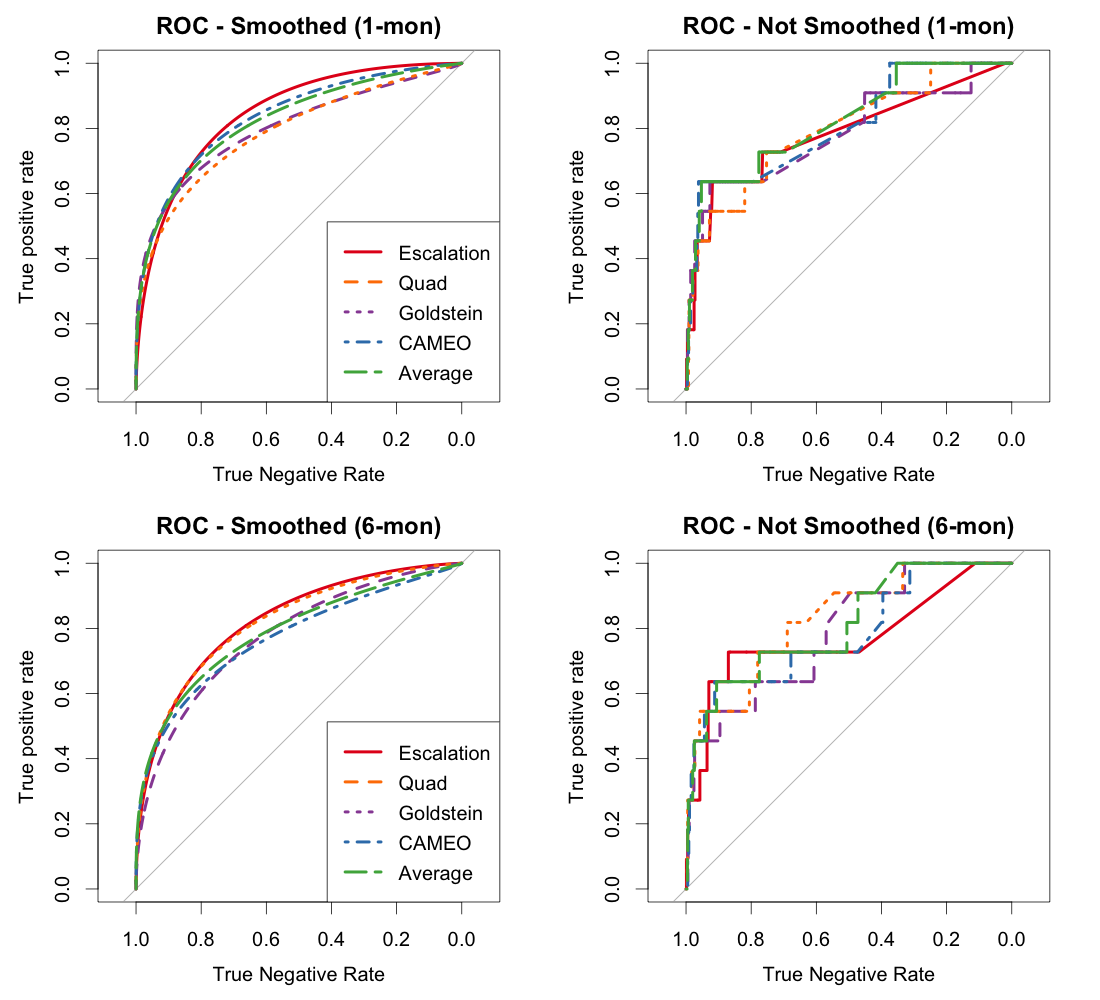
\includegraphics[width=.95\linewidth]{figures/fig-1-figure1-replicated.png}
\end{figure}

The specific predictions also include groups of cases with identical predicted probabilities, which accounts for the unusual diagonal lines seen in the panels on the right. In any case, with a sparse outcome like civil war onsets, the true positive rate on the \emph{y}-axis only changes when the prediction for an observed positive case is reached. For these ROC curves, and in the fundamental train/test split used for 12 of the 18 rows/models in B\&S Table 1, for that matter, there are only 11 civil war onset cases in the test set. Thus, the ROC curves here are very step-like, with only 12 (11 positive cases plus 1 for TPR = 0) distinct \emph{y} coordinates. Notice also that the smoothing averages the left-most almost straight line with the right-most almost straight line in a monotonic way. Thus, smoothing changes the ordering of alternatives. It is not a cosmetic change as suggested.

What impact did the ROC smoothing have overall on the evaluated performance of the Escalation model relative to other ICEWS models (our Table \ref{tab:table1-nosmooth}, B\&S Table 1) and structural extensions (our Table \ref{tab:table2-fixed}, B\&S Table 2)? Figure \ref{fig:benefit-plot} shows the changes in AUC-ROC values had we used smoothed ROC curves to calculate the AUC-ROC values. Each point corresponds to the change in AUC-ROC values for one of the models in the cells in Tables \ref{tab:table1-nosmooth} and \ref{tab:table2-fixed} (the colors match those in Figure \ref{fig:rocs}). The vertical bar in each plot marks the average effect of smoothing on AUC-ROC. For all alternative models, from Quad to ``PITF Only'', smoothing sometimes hurts and sometimes benefits, but the overall impact is negligible on average. The Escalation model, however, \emph{always} benefits from smoothing, with an average improvement on the order of 0.05. This is sufficient to push the Escalation model ahead of the alternative models and accounts for the incorrect result B\&S report, namely that the escalation model is generally superior.

\begin{figure}
\caption{Gain from using smoothed ROC to calculate AUC, for each model reported in Tables 3 and 4 (B\&S Tables 1 and 2). The Escalation model is the only model which consistently benefits from using smoothed ROC curves, and this advantage accounts for its apparent superiority to the other models.\label{fig:benefit-plot}}
\centering
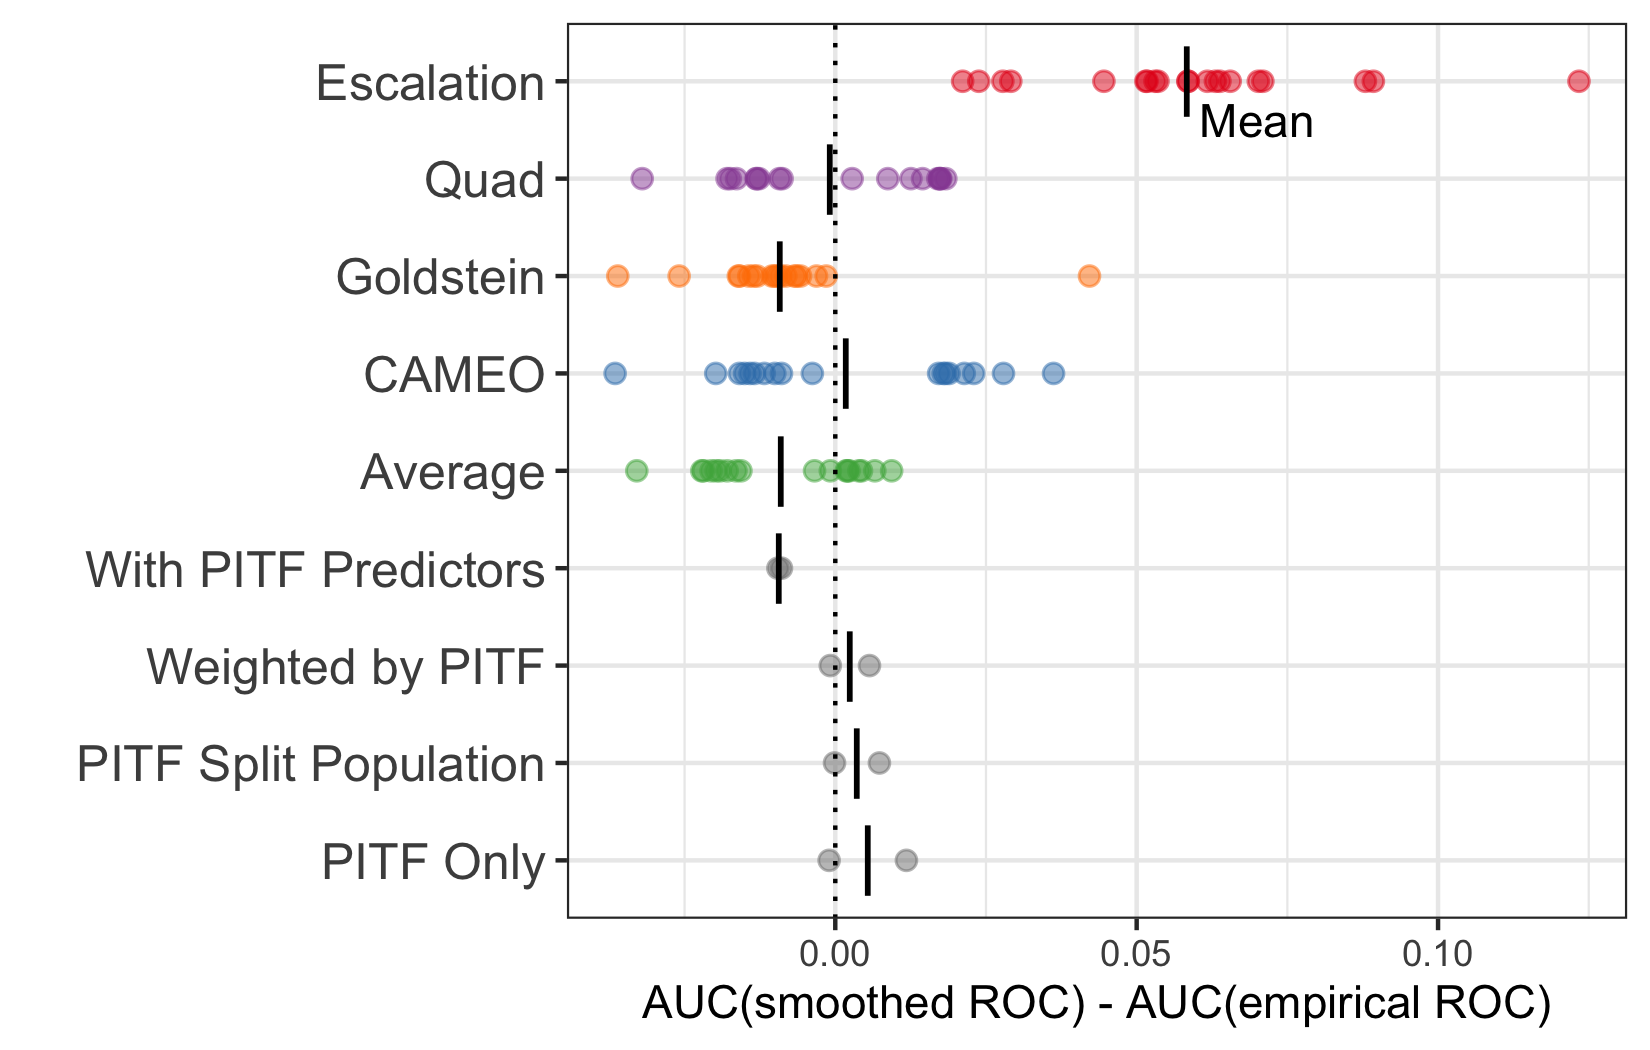
\includegraphics[width=.8\linewidth]{figures/fig-2-benefit-plot.png}
\end{figure}

In sum, it is not only the case that using smoothed ROC curves alters the results, but also that the use of smoothed ROC curves to calculate AUC-ROC values \textbf{only} benefits the escalation model. It does so consistently and by a considerable margin. All eight alternative models reported in B\&S Tables 1 and 2, on average, do not gain when using smoothed ROC curves to calculate AUC. Four of the eight show a small positive bias from smoothing, while the other four display a small negative bias. The magnitudes of these are not close to the level of positive bias found in the escalation model.

\hypertarget{is-the-escalation-model-superior-to-the-alternative-icews-models}{%
\subsection{Is the Escalation model superior to the alternative ICEWS models?}\label{is-the-escalation-model-superior-to-the-alternative-icews-models}}

Table \ref{tab:table1-nosmooth} (B\&S Table 1) shows the comparison of the Escalation model to other alternative models based on ICEWS event data indicators. The AUC-ROC values are based on original, non-smoothed ROC curves. Both the Average and the CAMEO models outperform the Escalation model in almost all instances (see also Figure \ref{fig:table1-plot}). The Goldstein model generally outperforms the Escalation model in the 6-month version. The Quad model appears to be roughly on par with the Escalation model. Thus, the original B\&S conclusion that the Escalation model is superior to the alternative models is entirely conditional on the non-standard use of smoothed ROC curves.

\begin{table}

\caption{\label{tab:table1-nosmooth}Comparison of the escalation model to alternative ICEWS model using test set AUC-ROC, \textit{without} smoothed ROC curves (Replication of B\&S Table 1)}
\centering
\begin{tabular}[t]{lrrrrr}
\toprule
Model & Escalation & Quad & Goldstein & CAMEO & Average\\
\midrule
\addlinespace[0.3em]
\multicolumn{6}{l}{\textbf{One-month forecasts}}\\
\hspace{1em}Base specification & 0.78 & 0.78 & 0.80 & 0.81 & 0.82\\
\hspace{1em}Terminal nodes & 0.79 & 0.78 & 0.79 & 0.81 & 0.82\\
\hspace{1em}Sample size & 0.79 & 0.80 & 0.74 & 0.82 & 0.84\\
\hspace{1em}Trees per forest & 0.78 & 0.78 & 0.79 & 0.81 & 0.82\\
\hspace{1em}Training/test sets 1 & 0.77 & 0.76 & 0.77 & 0.79 & 0.80\\
\hspace{1em}Training/test sets 2 & 0.75 & 0.77 & 0.74 & 0.76 & 0.78\\
\hspace{1em}Training/test sets 3 & 0.71 & 0.79 & 0.69 & 0.72 & 0.74\\
\hspace{1em}Coding of DV 1 & 0.80 & 0.80 & 0.80 & 0.82 & 0.83\\
\hspace{1em}Coding of DV 2 & 0.80 & 0.82 & 0.77 & 0.83 & 0.81\\
\addlinespace[0.3em]
\multicolumn{6}{l}{\textbf{Six-month forecasts}}\\
\hspace{1em}Base specification & 0.77 & 0.79 & 0.83 & 0.78 & 0.81\\
\hspace{1em}Terminal nodes & 0.77 & 0.78 & 0.82 & 0.78 & 0.79\\
\hspace{1em}Sample size & 0.77 & 0.77 & 0.80 & 0.80 & 0.82\\
\hspace{1em}Trees per forest & 0.77 & 0.79 & 0.83 & 0.79 & 0.81\\
\hspace{1em}Training/test sets 1 & 0.75 & 0.79 & 0.82 & 0.77 & 0.80\\
\hspace{1em}Training/test sets 2 & 0.70 & 0.75 & 0.78 & 0.75 & 0.77\\
\hspace{1em}Training/test sets 3 & 0.85 & 0.72 & 0.84 & 0.72 & 0.81\\
\hspace{1em}Coding of DV 1 & 0.78 & 0.80 & 0.83 & 0.79 & 0.82\\
\hspace{1em}Coding of DV 2 & 0.80 & 0.78 & 0.84 & 0.80 & 0.81\\
\bottomrule
\end{tabular}
\end{table}

The key difference between Table \ref{tab:table1-nosmooth} and B\&S Table 1 is whether the underlying ROC curves were original or smoothed; the test set N and coding issues did not affect this set of results.\footnote{We should note that in our replication we consciously decided to not set RNG seeds, even though the random forest models are non-deterministic and vary slightly from run to run. As we changed the replication code to allow running in parallel, we cannot exactly reproduce the B\&S results even with the same RNG seed. More importantly, the substantive interpretation of results should not depend on a specific RNG seed. We found that the escalation model's AUC-ROC values generally fluctuate no more than 0.01 (see \url{https://github.com/andybega/Blair-Sambanis-replication/blob/master/rep_nosmooth/variance.md}), and thus are confident that the patterns we see are robust to the initial RNG state.} B\&S's original results and interpretation regarding the superiority of the B\&S model over alternative ICEWS models, including the 1,000+ covariate CAMEO model, are thus entirely conditional on the use of smoothed AUC-ROC. Even the Quad model is generally as good as the escalation model in all implementations and is frequently quite a bit better.

Aside from the visual impact of ROC smoothing, the underlying motivation and methods involved in smoothing are broader and involve parametric estimation of population ROC curves (Hanley 1988, 2014). The main application is in the evaluation of medical tests (e.g.~diagnostic imaging) with early methods dating back several decades and ongoing development of both parametric and non-parametric smoothing methods (e.g.~Zou, Hall, and Shapiro 1997; Pulit 2016). It is not established which methods are preferable in a given application (Hanley 2014). Notably, the context in which ROC smoothing is used differs in important aspects from typical conflict research applications. Conflict data are closer to a census of the population and with well-known dependencies like spatial and temporal correlation, rather than a random sample that is approximately independently and identically distributed. It is thus neither clear that smoothing is justified nor valid. We also note that smoothed ROC plots are not widely used outside of the narrow context mentioned above.

\hypertarget{using-inconsistent-ns}{%
\subsection{Using Inconsistent Ns}\label{using-inconsistent-ns}}

The top portion of Table \ref{tab:table2-N} shows the number of valid test set predictions that can be scored for each model in the original B\&S Table 2. For the 1-month data version, the number of predictions differs by up to 500 cases, and in the 6-month data version by around 100 cases. These numbers appear small enough to be not important. However, the already small number of positive cases also is affected substantially: ``With PITF Predictors'' and ``PITF Only'' models lose two or one (respectively) of 11 positive cases in the 1- and 6-month data versions.

\begin{table}

\caption{\label{tab:table2-N}Number of valid test predictions for the escalation and structural alternatives models (B\&S Table 2)}
\centering
\begin{tabular}[t]{ll>{\raggedleft\arraybackslash}p{2cm}>{\raggedleft\arraybackslash}p{2cm}>{\raggedleft\arraybackslash}p{2cm}>{\raggedleft\arraybackslash}p{2cm}>{\raggedleft\arraybackslash}p{2cm}}
\toprule
 & Horizon & Escalation Only & With PITF Predictors & Weighted by PITF & PITF Split Population & PITF Only\\
\midrule
\addlinespace[0.3em]
\multicolumn{7}{l}{\textbf{Original model-specific cases}}\\
\hspace{1em} & 1 month & 13748 & 13155 & 13461 & 13748 & 13510\\
\cmidrule{2-7}
\hspace{1em} & 6 months & 2366 & 2264 & 2317 & 2366 & 2265\\
\cmidrule{1-7}
\addlinespace[0.3em]
\multicolumn{7}{l}{\textbf{Cases adjusted to common subset}}\\
\hspace{1em} & 1 month & 13062 & 13062 & 13062 & 13062 & 13062\\
\cmidrule{2-7}
\hspace{1em} & 6 months & 2250 & 2250 & 2250 & 2250 & 2250\\
\bottomrule
\end{tabular}
\end{table}

Generally, these comparisons require the same cases. Therefore, we use predictions for a common joint subset of non-missing predictions. The resulting numbers of cases for each model are shown in the bottom portion of the table. Since the sets of incomplete cases in the original version above do not entirely overlap themselves, the common subset for all models is slightly smaller than the smallest N in the top portion of the table.

\hypertarget{do-structural-variables-add-to-the-escalation-models-predictive-power}{%
\subsection{Do Structural Variables Add to the Escalation Model's Predictive Power?}\label{do-structural-variables-add-to-the-escalation-models-predictive-power}}

Table \ref{tab:table2-fixed} shows our replication of B\&S Table 2 with (1) regular, not smoothed, AUC-ROC, (2) fixed ``Weighted by PITF'' and ``PITF Split-Population'' models, and (3) AUC-ROC values computed on the common, joint subset of tests cases for which all models have non-missing predictions. Table \ref{tab:table2-full} in the appendix shows AUC-ROC values for both smoothed and non-smoothed versions, and both the original, model-varying test cases sets and our common joint subset.

\begin{table}

\caption{\label{tab:table2-fixed}Comparison of escalation model to structural extensions, using test set AUC-ROC (Replication of B\&S Table 2)}
\centering
\begin{threeparttable}
\begin{tabular}[t]{r>{\raggedleft\arraybackslash}p{2cm}>{\raggedleft\arraybackslash}p{2cm}>{\raggedleft\arraybackslash}p{2cm}>{\raggedleft\arraybackslash}p{2cm}>{}p{2cm}}
\toprule
Escalation Only & With PITF Predictors & Weighted by PITF & PITF Split Population & PITF Only\\
\midrule
\addlinespace[0.3em]
\multicolumn{5}{l}{\textbf{One-month forecasts}}\\
\hspace{1em}0.75 & 0.78 & 0.78 & 0.85 & 0.75\\
\addlinespace[0.3em]
\multicolumn{5}{l}{\textbf{Six-month forecasts}}\\
\hspace{1em}0.76 & 0.86 & 0.80 & 0.77 & 0.74\\
\bottomrule
\end{tabular}
\begin{tablenotes}[para]
\item \textit{Note: } 
\item Differences from the original B\&S Table 2: (1) AUC-ROC values are computed on the common subset of cases, meaning that N is equal in each row; (2) AUC-ROC values are computed using original, non-smoothed ROC curves.
\end{tablenotes}
\end{threeparttable}
\end{table}

B\&S interpret their results as follows (page 20) and we comment on the conclusions seriatim:\footnote{We list the ``Overall, \ldots{}'' interpretation out-of-order for clarity.}

\begin{enumerate}
\def\labelenumi{\arabic{enumi}.}
\tightlist
\item
  B\&S: ``Of the approaches we test, the split-population analog is most promising \ldots{}''
\end{enumerate}

The PITF split-population analog still performs well, but the simple Escalation + PITF predictors model performs better still.

\begin{enumerate}
\def\labelenumi{\arabic{enumi}.}
\setcounter{enumi}{1}
\tightlist
\item
  B\&S: ``Adding PITF predictors improves the performance of the escalation model over six-month windows but diminishes it over one-month windows \ldots ''
\end{enumerate}

Adding PITF predictors improves performance in both cases; the ``With PITF Predictions'' model strictly dominates the ``Escalation Only'' model by quite a margin in the 6-month data version.

\begin{enumerate}
\def\labelenumi{\arabic{enumi}.}
\setcounter{enumi}{2}
\tightlist
\item
  B\&S: ``The weighted model performs very poorly regardless \ldots ''
\end{enumerate}

The weighted model performs roughly on par with the Escalation Only model. One finding that remains is that the ``PITF Only'' model is outperformed by the ``Escalation Only'' model. As the former only uses annual inputs, but the data at hand are the 1-month or 6-months level, this is neither surprising nor especially noteworthy.

\begin{enumerate}
\def\labelenumi{\arabic{enumi}.}
\setcounter{enumi}{3}
\tightlist
\item
  B\&S: ``Overall, our results suggest that while measures of structural risk may improve predictive performance, the value they add is marginal and inconsistent. {[}\ldots{]} Incorporating PITF thus significantly reduces or only slightly improves the performance of the escalation model, regardless of the approach we take. {[}\ldots{]}''
\end{enumerate}

The most straightforward method of incorporating the annual structural PITF variables---adding them to the predictors of the Escalation RF model---strictly outperforms the Escalation Only model. Note that the two other combination models considered are both non-standard and that the ``PITF Split Population'' model does not incorporate structural information at all, yet they also both do well. We thus conclude that adding structural variables improves predictive performance.

\hypertarget{how-accurate-were-the-2016-forecasts}{%
\subsection{How Accurate Were the 2016 Forecasts?}\label{how-accurate-were-the-2016-forecasts}}

B\&S forecast the risk of civil war onset for the first half of 2016 (2016-H1, where H2 would be the second half), and assessed the accuracy of these forecasts. The forecasts themselves are probabilistic, i.e.~range from 0 to 1, but to score the forecasts they consider the 30 highest predictions to have been positive forecasts (``1'') and the remaining forecasts to have been for no onset (``0''). They evaluate two alternative codings of observed civil war outcomes, one in which 15 countries, including Colombia, had ongoing civil wars at the end of 2015 (labeled ``Assuming Persistence''), and an alternative coding in which the civil war in Colombia ends but Turkey and Benin experience civil war onsets (``Assuming Change'').\footnote{\label{fn:leadDV}The former coding is in the main replication data, while the latter is hand-coded in the Stata script that produces their confusion matrices. There is also some potential ambiguity about the discussion in this section because the forecasts B\&S claim are for the first half of 2016 are actually for the second half of 2016, but scored against outcomes for the first half of 2016.} However, when they score the forecasts to produce the confusion matrices they report in their Table 4, they score them using civil war incidence, not onset. This a conscious choice B\&S acknowledge in the text (if not the table with confusion matrices), but it's not clear to us how this is justifiable.

For reference for the following discussion, we reproduce confusion matrices for the 2016-H1 forecasts in Table \ref{tab:table4}, but distinguish between civil war onsets (\(Y=1\)), non-events (\(Y=0\)) that correspond to countries with an ongoing civil war, and non-events (\(Y=0\)) that correspond to countries without a civil war, but which could potentially experience a civil war onset. The original B\&S confusion matrices collapse the second two rows in each matrix and treat ongoing and onset as part of the same group. Essentially, all of the apparent true positives (\(P=1, Y=1\)) in the original B\&S confusion matrices are ongoing civil war cases which by definition \emph{cannot} experience another civil war onset. The alternative outcome coding B\&S evaluate, under ``Assuming Change'', produces the only two civil war onsets we would have observed in 2016-H1.

\begin{table}
\caption{Replication of B\&S Table 4: Confusion Matrices for Six-month Escalation Model forecasts for the first half of 2016.}\label{tab:table4}
\centering
\begin{tabular}{ll|c|c|l}
\multicolumn{1}{l}{\multirow{5}{*}{Assuming Persistence}} & \multicolumn{3}{c}{} \\
\multicolumn{2}{c}{}& \multicolumn{1}{c}{$P=0$} & \multicolumn{1}{c}{$P=1$} \\
\cline{3-4}
& $Y=0$, no civil war & 134 & 17 \\
\cline{3-4}
& $Y=0$, ongoing & 2 & 13 \\
\cline{3-4}
& $Y=1$, onset & 0 & 0 \\
\cline{3-4}
% fixed, assuming change
\multicolumn{1}{l}{\multirow{5}{*}{Assuming Change}} & \multicolumn{3}{c}{} \\
\multicolumn{2}{c}{}& \multicolumn{1}{c}{$P=0$} & \multicolumn{1}{c}{$P=1$} \\
\cline{3-4}
& $Y=0$, no civil war & 134 & 16 \\
\cline{3-4}
& $Y=0$, ongoing & 2 & 12 \\
\cline{3-4}
& $Y=1$, onset & 0 & 2 \\
\cline{3-4}
\\
\end{tabular}
\end{table}

The fact that countries with an ongoing civil war cannot experience another civil war onset follows from the way the Sambanis civil war data conceptualize and operationalize civil war. Civil war appears to be a binary property of a country at any given moment in time, i.e.~a country at any given point is either at civil war or not, and onset is the first time period corresponding to this state. In the data, ongoing civil wars are coded as having a missing outcome value and dropped.

If we place ourselves back to the beginning of 2016, when the forecasts were made (the forecasts are pre-registered in early March), this means that we would have observed that 15 countries had ongoing conflicts in the second half of 2015 which had not terminated prior to the forecasting period. In all previous analyses in the paper, these kinds of cases drop out of the data. However, B\&S re-introduce, produce forecasts for them, and include them as positive events (``1''s) in their confusion matrices. They write, on page 21:

\begin{quote}
Importantly, we make no assumptions about the persistence of civil war between the second half of 2015 and the first half of 2016, meaning that all countries---even those with ongoing conflicts as of December 31, 2015---are included in the 2016 test set. As a result, 14 of the 30 countries on the list (and nine of the top 10) are cases of ongoing conflict.
\end{quote}

It's not clear to us under what conditions forecasting civil war onset risk for countries with ongoing civil wars make sense. A
conflict could have ended in 2015-H2 and a new one started right away in 2016-H1, but when making the forecasts, \emph{we would have already known that}. Rather than not making any ``assumptions about the persistence of civil war'', this would only make sense if we assume that all ongoing civil wars ended in 2015-H2. Since Sambanis is the author of the civil war data that is used, it would already have been known in early 2016 that these 15 civil wars had not terminated, and were still ongoing. It is thus both by definition impossible for countries with ongoing civil wars to experience another onset, and at the time the forecasts were made it would have been known that all conflicts were still ongoing up through the beginning of the forecasting period.

Does it make sense to count a high probability for the risk of onset for a case with an ongoing civil war as a partial or complete ``win'' for the model? When creating the confusion matrices, B\&S treat these ongoing civil war instances equivalent to civil war onsets, as positive events (``1''). In the text, B\&S do acknowledge a distinction between predicting an actual onset versus predicting a continuation, but they also claim credit for the fact that the model places high probabilities on most of the ongoing civil war cases. This would only make sense if the civil war coding was at the conflict, not country-level, so that a country could experience more than one civil war at any given time, e.g., two separatists' conflicts in different portions of the country. But this is not the case; ongoing conflicts in all other analyses are consistently dropped from the data as if a new civil war onset for a country with an ongoing conflict is conceptually impossible.

If we turn back to the confusion matrices to re-assess the accuracy of the 2016-H1 forecasts, we can thus conclude that almost all of the predictions are false positives. There are no onsets in the ``Assuming Persistence'' coding, and two onsets in the ``Assuming Change'' coding. This is normal. Civil war onsets are infrequent, and it is to be expected that forecasts of rare events will mostly consist of false positives. The forecasts do correctly capture the 2 civil war onsets in the ``Assuming Change'' version of the outcome coding. This is, at face value, a credit to the model's accuracy.

\hypertarget{discussion}{%
\section{Discussion}\label{discussion}}

B\&S advocate the use of theory to guide prediction. But ``theory'' is not defined by B\&S and may be an ambiguous and undefined concept. ``Theory'' has many interpretations in social science. For some---the EITM movement, for example (Aldrich, Alt, and Lupia 2008)---theory is a system of internally consistent, logically connected propositions from which additional statements may be deduced. The additional statements can be subjected to empirical scrutiny. An example might be William Riker's theory of coalitions (Riker 1962) which posits propositions in game-theoretic form from which the size principle of minimal winning coalitions may be deduced and further examined empirically. A more recent example of strong theory is found in \emph{The Political Logic of Survival} (Bueno de Mesquita et al. 2005). For the purposes of discussion, we call this strong theory.

However, for many, a theory is simply a falsifiable story or narrative that makes causal claims about the relationships among variables. Typically, it is fused together from a meta-analysis of prior work on the topic under consideration. We call these types of theory weak theory. They are weak because they do not include two characteristics of strong theory, though they may include one:

\begin{enumerate}
\def\labelenumi{\arabic{enumi}.}
\tightlist
\item
  A theory is separate from the case or cases being examined. It is intended to be general.
\item
  A theory generates new statements that in principle can be empirically falsified, not proven.
\end{enumerate}

Most social science research uses a weak form of theory. In the case of B\&S they base their theoretical thinking on research that argues that conflict is not the product of structural factors, but rather comes from an interaction of state repression and the changes in costs and benefits to citizens for engaging in anti-government conflict. Following a wide swath of scholars, they argue that the escalation and de-escalations of interactions between citizens and government are what typically lead up to the onset of civil wars. Operationally, this boils down to four types of concepts: demands, accommodations, nonviolent repression, and low-level violence.

\begin{itemize}
\item Demands include events in which either opposition or rebels is the source and government is the target and typically involve appeals for political or institutional reform, policy change, or extension of rights.
\item Nonviolent repression and accommodation include events in which the government is the source and either opposition or rebels is the target. Nonviolent repression includes threats, sanctions, restrictions on freedom of movement, or rejections of group demands.
\item Low-level violence includes all events in which (1) the government is the source and opposition is the target, (2) the opposition is the source and government is the target, (3) the government is the source and rebels are the target, or (4) rebels are the source and government is the target.
\end{itemize}

These variables, taken from ICEWS, are the main components of the escalation model in the B\&S article. The escalation theory is that the forces behind these variables interact such that as each of them increases, they independently increase the probability of civil conflict. The actual mechanisms of the dynamism among these variables are not specified.

Indeed, most empirical social science research follows this approach: (1) delineation of an argument, (2) selection of variables that represent a plausible or compelling representation of the concepts, followed by (3) utilization of these variables in a statistical model with a dependent variable that measures the main phenomena of investigation. It is worth pointing out that this is simply one set of variables that are selected to represent the concepts in the theoretical story.

A strong theory gives more guidance on compelling choices than does a weak theory. Accordingly, while the choice is plausible, it is not necessarily compelling. Another choice might be equally plausible. In the ICEWS example, we might include variables on intragovernmental demands (from the military toward the central government), or further look at the dynamics among opposition groups. In practical terms, there is a wide array of choices that are available to instantiate any particular theory. A second point is that putting them in a linear regression may be a particularly crude instantiation of complicated dynamics. One general principle in the B\&S article that is on point, and is more widely relevant, is that dynamical phenomena like civil wars need to have explanatory models that change rapidly over time---and by implication that are represented by data that change fairly quickly.

Instantiating the theoretical model is more about choosing the correct variables. This is the contrast between theoretical prediction models and atheoretical machine learning that B\&S focus on. But this dichotomy is misguided. The data that are used in a predictive model have to come from somewhere. Even if the inclusion of some factors is not explicitly justified, it is hardly the case that one assembles data without the expectation that it will be useful. It is not a coincidence that nobody uses 1,180 variable strawman models whose variable vectors predominantly consist of 0's, even if such a model coincidentally ends up performing well. Rather, we posit that most of the cases B\&S might characterize as atheoretical enter the ``theoretical'' with some awareness of existing arguments and work that is used to select data sources for inclusion in a dataset.\footnote{While we do not undertake this, there are a variety of procedures that one might use for variable choices, ranging from staring at lists of variables to machine learning approaches.}

Furthermore, if what we mean by the concept ``theory'' is such that it suggests a large range of variables that could be related to an outcome, what do we really gain from having this theory in our predictive model? We can construct a model designed to predict well while avoiding overfitting, and then go back and try to couch it in theoretical language---which, given the malleability of extant theory, we probably could in many cases---but are we then better off? Certainly, that's not what B\&S are trying to suggest since this would be a problematic way to ``evaluate'' a theory. But when theory is extensive or malleable so that it suggests a broad range of variables and specifications, and thus a broad range of specifications could, in fact, be tied to a theory, it is hard to demonstrate that this theory is not the result of predictive modeling's equivalent to p-hacking, namely developing a model specification and associated ``theory'' with an eye towards out-of-sample predictive accuracy (cf.~Colaresi and Mahmood 2017 for how to avoid this problem while leveraging out-of-sample predictions). Incidentally, this is also a recipe for creating overfit models whose accuracy does not generalize and whose underlying theories may by extension not be externally valid (for a more detailed treatment of this issue, see Fariss and Jones 2018).

Conversely, not all factors that are ``theoretically'' important or suggested by the literature are also important for prediction, and some factors that are good predictors do not originate from prior theory. For example, both Ward, Greenhill, and Bakke (2010) and Hill and Jones (2014) examine a variety of variables that are considered ``theoretically'' important for explaining civil war onset and state repression, respectively, and find that there is substantial variation in how useful they are for actually predicting those outcomes. It is also possible that building accurate predictive models could uncover factors overlooked in the literature, e.g., the strong association between infant mortality and a broad variety of conflict outcomes like political instability (Goldstone et al. 2010), irregular leadership changes (Beger et al. 2017), and coups (Beger and Ward 2020).

Aside from the selection of the variables that go into a model, another way in which we could contrast theoretical from atheoretical prediction models is in terms of their flexibility regarding functional form. Theory should not only tell us what factors matter, but also how they relate to each other. We think that few would be strongly committed to the idea that the linear additive equations that dominate published regression analyses, maybe with the occasional polynomial or multiplicative interaction terms, are \emph{the} correct functional specification. Is the danger posed by low-level violence the same when tensions are high, with high demands and high non-violent repression, as when tensions are low? Are those relationships linear in the log-odds? Some machine learning models, random forests included, are flexible in this regard and, to some extent, are capable of learning non-linear and interactive relationships. B\&S implicitly concede on this point since they use random forests for both their Escalation model and the atheoretical alternatives. But in the absence of strong a priori theoretical expectations about functional form, why not use machine learning tools to try to uncover any such non-linear relationships in need of explanation, and use this to improve our theory (see also Fariss and Jones 2018)?

Rather than trying to frame theoretical modeling and machine learning as competing endeavors, a more useful perspective is to consider how they can mutually reinforce each other. Even if the analysis in B\&S fails to support the point, we concede that predicting on the basis of a strong theoretical model is preferable to inductive prediction. Beyond accurate predictions, such models would allow us to make causal statements that are harder to make on the basis of ad hoc models. But this is hard to do in practice. The problem is that many extant theoretical models are in fact so malleable to interpretation that they essentially are ad hoc. They are useful for identifying variables that could be useful for prediction, and this is already taking place.

Most importantly, a single study is unlikely to be convincing that theory-based models are better (or worse) than ad hoc models based on machine learning. Even if B\&S were correct that in their study the theory-based escalation model performed better, it would simply be a case study of a single case where it was preferable. It establishes no general tendency, let alone law-like evidence for general theory. Nor, against it.

\hypertarget{conclusion}{%
\section{Conclusion}\label{conclusion}}

We encountered several issues in the code underlying the B\&S analysis. The problems we encountered are not subjective modeling choices. They bear no implications on the question of whether theory-based models are preferable. However, when we fix these issues and perform an updated analysis, the B\&S conclusions are all essentially overturned. In other words, B\&S findings are based on a faulty analysis, invalid, and should be disregarded as evidence in favor of theory-based models.

In contradistinction to the conclusions offered by B\&S, we find that when correctly specified and implemented:

\begin{itemize}
\tightlist
\item
  The theory-driven escalation model is outperformed both by the low-effort 1,160 predictor all-CAMEO model and the ensemble average model.
\item
  The Average ensemble model and the CAMEO models outperform the escalation model in all instances.
\item
  Adding structural variables substantially improves the escalation model's performance.
\end{itemize}

More importantly, trying to contrast machine learning and theory may be misguided. Even if a ``theory'' section is missing, predictive models are informed by previous work and arguments. If we had strong general theories of something like civil war onset, we could replace more inductive, ad hoc, methods with clearly specified models. But we do not. What we have instead are weak theories that could be interpreted to suggest any range of equations for predicting an outcome. Instead of trying to find an instantiation of such a ``theoretical'' model that can outperform a more ad hoc alternative, we could use the flexibility of machine learning methods and insights that predictive modeling brings to improve our weak theories.

Blair \& Sambanis have focused attention on comparing forecasting models and forecasts in the civil war domain. As social science becomes more adept at predictive analysis, this will doubtless be of increasing importance. However, these comparisons must be made carefully to ensure those correct inferences are drawn. We continue to think that weak theory is overrated (Ward 2016) and that machine learning and big data will allow us to learn new things. It will be interesting to see how the evidence for these claims is adjudicated with additional usage and careful evaluation. Social science has leaned on theory for (at least) seventy years, but it is time to find useful ways to incorporate recently developed methods in the arena of machine learning and modern statistics.

\newpage

\hypertarget{references}{%
\section{References}\label{references}}

\hypertarget{refs}{}
\begin{cslreferences}
\leavevmode\hypertarget{ref-aldrich:etal:2008}{}%
Aldrich, John H., James E. Alt, and Arthur Lupia. 2008. ``The Eitm Approach: Origins and Interpretations.'' In \emph{The Oxford Handbook of Political Methodology}.

\leavevmode\hypertarget{ref-beger:etal:2017}{}%
Beger, Andreas, Daniel W. Hill, Jr., Nils. W. Metternich, Shahryar Minhas, and Michael D. Ward. 2017. ``Splitting It Up: The \texttt{spduration} Split-Population Duration Regression Package for Time-Varying Covariates.'' \emph{The \(\mathcal{R}\) Journal} 9 (2): 474--86. \url{https://journal.r-project.org/archive/2017/RJ-2017-056/index.html}.

\leavevmode\hypertarget{ref-beger:etal:2020}{}%
Beger, Andreas, Richard K. Morgan, and Laura Maxwell. 2020. ``The Democratic Spaces Barometer: Global Forecasts of Autocratization and Democratization.'' \url{https://www.v-dem.net/en/analysis/DemSpace/}.

\leavevmode\hypertarget{ref-beger:ward:2017}{}%
Beger, Andreas, and Michael D. Ward. 2017. ``Lessons from Near Real-Time Forecasting of Irregular Leadership Changes.'' \emph{Journal of Peace Research} 54 (2): 141--56.

\leavevmode\hypertarget{ref-beger:ward:2020}{}%
---------. 2020. ``Coup Forecasts for 2020.'' \url{https://www.predictiveheuristics.com/forecasts}.

\leavevmode\hypertarget{ref-blair:sambanis:2020}{}%
Blair, Robert A., and Nicholas Sambanis. n.d. ``Forecasting Civil Wars: Theory and Structure in an Age of `Big Data' and Machine Learning.'' \emph{Journal of Conflict Resolution} TBD (firstview): 0022002720918923.

\leavevmode\hypertarget{ref-breiman:2001}{}%
Breiman, Leo. 2001. ``Random Forests.'' \emph{Machine Learning} 45 (1): 5--32.

\leavevmode\hypertarget{ref-bdm:etal:2005}{}%
Bueno de Mesquita, Bruce, Alastair Smith, Randolph M. Siverson, and James D. Morrow. 2005. \emph{The Logic of Political Survival}. Cambridge, Mass: MIT Press.

\leavevmode\hypertarget{ref-cederman:weidmann:2017}{}%
Cederman, Lars-Erik, and Nils B. Weidmann. 2017. ``Predicting Armed Conflict: Time to Adjust Our Expectations?'' \emph{Science} 355 (6324): 474--76.

\leavevmode\hypertarget{ref-chiba:etal:2015}{}%
Chiba, Daina, Nils W. Metternich, and Michael D. Ward. 2015. ``Every Story Has a Beginning, Middle, and an End (but Not Always in That Order): Predicting Duration Dynamics in a Unified Framework.'' \emph{Political Science Research and Methods} 3 (3): 515--41.

\leavevmode\hypertarget{ref-colaresi:mahmood:2017}{}%
Colaresi, Michael, and Zuhaib Mahmood. 2017. ``Do the Robot: Lessons from Machine Learning to Improve Conflict Forecasting.'' \emph{Journal of Peace Research} 54 (2): 193--214.

\leavevmode\hypertarget{ref-fariss:jones:2018}{}%
Fariss, Christopher J., and Zachary M. Jones. 2018. ``Enhancing Validity in Observational Settings When Replication Is Not Possible.'' \emph{Political Science Research and Methods} 6 (2): 365--80.

\leavevmode\hypertarget{ref-goldstone:etal:2010}{}%
Goldstone, Jack A., Robert H. Bates, David L. Epstein, Ted Robert Gurr, Michael B. Lustik, Monty G. Marshall, Jay Ulfelder, and Mark Woodward. 2010. ``A Global Model for Forecasting Political Instability.'' \emph{American Journal of Political Science} 54 (1): 190--208.

\leavevmode\hypertarget{ref-henley:1988}{}%
Hanley, James A. 1988. ``The Robustness of the "Binormal" Assumptions Used in Fitting ROC Curves.'' \emph{Medical Decision Making} 8 (3): 197--203. \url{https://doi.org/10.1177/0272989X8800800308}.

\leavevmode\hypertarget{ref-henley:2014}{}%
---------. 2014. ``Receiver Operating Characteristic (ROC) Curves.'' In \emph{Wiley Statsref: Statistics Reference Online}. American Cancer Society. \url{https://doi.org/10.1002/9781118445112.stat05255}.

\leavevmode\hypertarget{ref-hegre:etal:2019}{}%
Hegre, Håvard, Marie Allansson, Matthias Basedau, Michael Colaresi, Mihai Croicu, Hanne Fjelde, Frederick Hoyles, et al. 2019. ``ViEWS: A Political Violence Early-Warning System.'' \emph{Journal of Peace Research} 56 (2): 155--74.

\leavevmode\hypertarget{ref-hill:jones:2014}{}%
Hill, Daniel W., and Zachary M. Jones. 2014. ``An Empirical Evaluation of Explanations for State Repression.'' \emph{American Political Science Review} 108 (03): 661--87.

\leavevmode\hypertarget{ref-liaw:wiener:2002}{}%
Liaw, Andy, and Matthew Wiener. 2002. ``Classification and Regression by randomForest.'' \emph{R News} 2 (3): 18--22. \url{https://CRAN.R-project.org/doc/Rnews/}.

\leavevmode\hypertarget{ref-malley:etal:2012}{}%
Malley, James D., Jochen Kruppa, Anirban DasGupta, Karen G. Malley, and Andreas Ziegler. 2012. ``Probability Machines: Consistent Probability Estimation Using Nonparametric Learning Machines.'' \emph{Methods of Information in Medicine} 51 (1): 74--81. \url{https://www.thieme-connect.de/products/ejournals/abstract/10.3414/ME00-01-0052}.

\leavevmode\hypertarget{ref-pulit:2016}{}%
Pulit, Michał. 2016. ``A New Method of Kernel-Smoothing Estimation of the Roc Curve.'' \emph{Metrika} 79 (5): 603--34.

\leavevmode\hypertarget{ref-riker:1962}{}%
Riker, William H. 1962. \emph{The Theory of Political Coalitions}. Yale University Press.

\leavevmode\hypertarget{ref-ward:2016}{}%
Ward, Michael D. 2016. ``Can We Predict Politics? Toward What End?'' \emph{Journal of Global Security Studies} 1 (1): 80--91.

\leavevmode\hypertarget{ref-ward:etal:2010}{}%
Ward, Michael D., Brian D. Greenhill, and Kristin M. Bakke. 2010. ``The Perils of Policy by P-Value: Predicting Civil Conflicts.'' \emph{Journal of Peace Research} 47 (4): 363--75.

\leavevmode\hypertarget{ref-ward:etal:2013}{}%
Ward, Michael D., Nils W. Metternich, Cassy L. Dorff, Max Gallop, Florian M. Hollenbach, Anna Schultz, and Simon Weschle. 2013. ``Learning from the Past and Stepping into the Future: Toward a New Generation of Conflict Prediction.'' \emph{International Studies Review} 16 (4): 473--644.

\leavevmode\hypertarget{ref-zou:etal:1997}{}%
Zou, Kelly H., William J. Hall, and David E. Shapiro. 1997. ``Smooth Non-Parametric Receiver Operating Characteristic (ROC) Curves for Continuous Diagnostic Tests.'' \emph{Statistics in Medicine} 16 (19): 2143--56.
\end{cslreferences}

\newpage

\hypertarget{appendix-appendix}{%
\appendix}


\hypertarget{appendix}{%
\section{Appendix}\label{appendix}}

\renewcommand{\thefigure}{A\arabic{figure}}
\setcounter{figure}{0}

\renewcommand{\thetable}{A\arabic{table}} 
\setcounter{table}{0}

\hypertarget{code-references-for-coding-errors}{%
\subsection{Code references for coding errors}\label{code-references-for-coding-errors}}

\hypertarget{section-3.2-incorrect-weighted-by-pitf-implementation}{%
\subsubsection{Section 3.2: Incorrect ``Weighted by PITF'' Implementation}\label{section-3.2-incorrect-weighted-by-pitf-implementation}}

We believe the intention with the ``Weighted by PITF'' model is to combine the PITF test predictions with the Escalation test predictions, i.e.~weight the latter with the former. Due to an error, the PITF \emph{training} set predictions are used, not the \emph{test} set predictions.

See \texttt{1mo\_run\_escalation\_weighted\_PITF.R} line 4, where the PITF predictions are taken from the training data set (\texttt{train\$pred\_prob\_plus1}). The next line is a hack extending the shorter \texttt{weight} vector with missing values to avoid a R warning when it is multiplied with the longer vector of escalation model test set predictions -- similarly in the 6-month version of this file.

Uncovering which cases in the PITF training predictions are matched to the cases that the Escalation model test set predictions correspond to requires tracing back several more data objects. We have documented details in issue \#3 in the GitHub repo.

\hypertarget{section-3.3-incorrect-pitf-split-population-implementation}{%
\subsubsection{Section 3.3: Incorrect ``PITF Split Population'' Implementation}\label{section-3.3-incorrect-pitf-split-population-implementation}}

The intention is to train separate random forests on data split into high and low-risk groups based on PITF predictions, and then combine them back into one random forest. Actually, both random forests are trained on identical data, essentially production a random forest that just has N\_trees * 2.

Disentangling this coding error is not straightforward as it occurs over several R scripts and requires (or at least is easier to verify by) running partway through the actual replication until the objects holding the training data for the models are instantiated and can be examined. Details are documented in issue \#5 in the GitHub repo.

\hypertarget{section-3.5-incorrect-scoring-of-the-2016-forecasts}{%
\subsubsection{Section 3.5: Incorrect scoring of the 2016 forecasts}\label{section-3.5-incorrect-scoring-of-the-2016-forecasts}}

Regarding the claim in footnote \ref{fn:leadDV} that the 2016-H1 forecasts are actually forecasts for 2016-H2:

\begin{enumerate}
\def\labelenumi{\arabic{enumi}.}
\tightlist
\item
  Throughout the R code for the main analyses, the models predict a 1-time period lead version of the civil war onset variables (ending in "\_plus1``). This means that, for example, in the 6-month version of the data, a value of''1" for the "\_plus1" outcome variable for 2015-H2 actually refers to a civil war onset in the first half of 2016. One can confirm, through some tracing to work back to the original variable assignments, that the ROC curves and AUC are correspondingly, and correctly, also scored using the lead versions of the DV.
\item
  The nominally 2016-H1 forecasts are created at the bottom of \texttt{+master.R} using the data for 2016-H1 and still the lead DV. Thus, the lead DV here refers to outcomes in 2016-H2.
\item
  The scoring of the forecasts, whatever time period they are actually for, is done in a separate Stata do file, \texttt{6mo\_make\_confusion\_matrix.do}. Here, the scoring is done using the non-lead version of the DV. Thus, there is a mismatch between the time period the forecasts are for and the period whose observed outcomes are used to score them.
\end{enumerate}

The relevant variables in the data are ``incidence\_civil\_ns'' and ``incidence\_civil\_ns\_plus1'', which appears to be a 1-period lead (i.e., \(t_{+1}\)) version of the dependent variable that is used in the actual prediction models. The incidence dependent variable contains both 0/1 and missing values. By examining the pattern of missing values, it seems clear that this was originally an incidence variable indicating whether a country was at civil war in a given year or not, and which was converted to an onset version so that onsets retain the value of 1 but continuing civil war years are coded as missing. This reflects common practice.

Furthermore, by examining the code used to generated Table 4, we were able to confirm that the onset forecasts are assessed using incidence, not onset. In the file \texttt{6mo\_make\_confusion\_matrix.do} on line 52, missing values in ``incidence\_civil\_ns'' are recoded to 1, thus reverting the onset coding of this variable to incidence.

\hypertarget{additional-replication-tables}{%
\subsection{Additional replication tables}\label{additional-replication-tables}}

Table \ref{tab:table1-smooth} is our replication of B\&S Table 1 with smoothed AUC-ROC. The results differ slightly from the original B\&S Table 1, typically by no more than 0.01, due to the non-deterministic nature of the RF models. It is the case that B\&S set the RNG seed in their replication code, which should theoretically allow exact reproduction, but (1) there was a change in more recent versions of R that affected the RNG seeding process, and (2) we refactored the replication script to allow one to run the models in parallel. In any case, the interpretation of results should not be sensitive to random variation, i.e.~it should not depend on using a specific RNG seed. On the basis of these results, B\&S conclude that the escalation model is generally superior to the alternatives, and we can replicate that interpretation when using smoothed ROC curves.

\begin{table}

\caption{\label{tab:table1-smooth}Replication of B\&S Table 1 with smoothed ROC curves; test set AUC-ROC for various models}
\centering
\begin{tabular}[t]{lrrrrr}
\toprule
Model & Escalation & Quad & Goldstein & CAMEO & Average\\
\midrule
\addlinespace[0.3em]
\multicolumn{6}{l}{\textbf{One-month forecasts}}\\
\hspace{1em}Base specification & 0.85 & 0.80 & 0.79 & 0.84 & 0.83\\
\hspace{1em}Terminal nodes & 0.86 & 0.79 & 0.77 & 0.83 & 0.82\\
\hspace{1em}Sample size & 0.85 & 0.81 & 0.71 & 0.86 & 0.84\\
\hspace{1em}Trees per forest & 0.85 & 0.80 & 0.78 & 0.83 & 0.82\\
\hspace{1em}Training/test sets 1 & 0.86 & 0.78 & 0.76 & 0.81 & 0.80\\
\hspace{1em}Training/test sets 2 & 0.82 & 0.79 & 0.72 & 0.77 & 0.78\\
\hspace{1em}Training/test sets 3 & 0.80 & 0.80 & 0.69 & 0.74 & 0.75\\
\hspace{1em}Coding of DV 1 & 0.86 & 0.81 & 0.80 & 0.84 & 0.83\\
\hspace{1em}Coding of DV 2 & 0.92 & 0.80 & 0.81 & 0.81 & 0.81\\
\addlinespace[0.3em]
\multicolumn{6}{l}{\textbf{Six-month forecasts}}\\
\hspace{1em}Base specification & 0.82 & 0.78 & 0.82 & 0.77 & 0.79\\
\hspace{1em}Terminal nodes & 0.79 & 0.76 & 0.81 & 0.77 & 0.77\\
\hspace{1em}Sample size & 0.83 & 0.78 & 0.78 & 0.79 & 0.79\\
\hspace{1em}Trees per forest & 0.82 & 0.77 & 0.82 & 0.77 & 0.79\\
\hspace{1em}Training/test sets 1 & 0.80 & 0.78 & 0.81 & 0.76 & 0.78\\
\hspace{1em}Training/test sets 2 & 0.72 & 0.74 & 0.77 & 0.73 & 0.75\\
\hspace{1em}Training/test sets 3 & 0.88 & 0.71 & 0.81 & 0.68 & 0.79\\
\hspace{1em}Coding of DV 1 & 0.83 & 0.77 & 0.82 & 0.79 & 0.80\\
\hspace{1em}Coding of DV 2 & 0.83 & 0.77 & 0.83 & 0.78 & 0.79\\
\bottomrule
\end{tabular}
\end{table}

\begin{table}

\caption{\label{tab:table2-full}Replication of B\&S Table 2 with smoothed/original ROC and with original varying N cases or adjusting for common case set with constant N}
\centering
\begin{tabular}[t]{ll>{\raggedright\arraybackslash}p{1.5cm}>{\raggedleft\arraybackslash}p{2cm}>{\raggedleft\arraybackslash}p{2cm}>{\raggedleft\arraybackslash}p{2cm}>{\raggedleft\arraybackslash}p{2cm}>{\raggedleft\arraybackslash}p{2cm}}
\toprule
 &  & Smoothed ROC & Escalation Only & With PITF Predictors & Weighted by PITF & PITF Split Population & PITF Only\\
\midrule
\addlinespace[0.3em]
\multicolumn{8}{l}{\textbf{Original model-specific cases}}\\
\addlinespace[0.3em]
\multicolumn{8}{l}{\textit{1 month}}\\
\hspace{1em}\hspace{1em} &  & Yes & 0.85 & 0.77 & 0.80 & 0.81 & 0.76\\
\cmidrule{3-8}
\hspace{1em}\hspace{1em} &  & No & 0.79 & 0.78 & 0.80 & 0.79 & 0.75\\
\cmidrule{2-8}
\addlinespace[0.3em]
\multicolumn{8}{l}{\textit{6 months}}\\
\hspace{1em}\hspace{1em} &  & Yes & 0.82 & 0.85 & 0.81 & 0.78 & 0.74\\
\cmidrule{3-8}
\hspace{1em}\hspace{1em} &  & No & 0.77 & 0.86 & 0.81 & 0.78 & 0.74\\
\cmidrule{1-8}
\addlinespace[0.3em]
\multicolumn{8}{l}{\textbf{Cases adjusted to common subset}}\\
\addlinespace[0.3em]
\multicolumn{8}{l}{\textit{1 month}}\\
\hspace{1em}\hspace{1em} &  & Yes & 0.81 & 0.77 & 0.79 & 0.86 & 0.76\\
\cmidrule{3-8}
\hspace{1em}\hspace{1em} &  & No & 0.75 & 0.78 & 0.78 & 0.85 & 0.75\\
\cmidrule{2-8}
\addlinespace[0.3em]
\multicolumn{8}{l}{\textit{6 months}}\\
\hspace{1em}\hspace{1em} &  & Yes & 0.82 & 0.85 & 0.80 & 0.77 & 0.74\\
\cmidrule{3-8}
\hspace{1em}\hspace{1em} &  & No & 0.76 & 0.86 & 0.80 & 0.77 & 0.74\\
\bottomrule
\end{tabular}
\end{table}

\begin{table}

\caption{\label{tab:table1-benefit}Smoothing advantage for B\&S Table 1: the gain in AUC-ROC when calculated using smoothed ROC curves}
\centering
\begin{tabular}[t]{lrrrrr}
\toprule
Model & Escalation & Quad & Goldstein & CAMEO & Average\\
\midrule
\addlinespace[0.3em]
\multicolumn{6}{l}{\textbf{One-month forecasts}}\\
\hspace{1em}Base specification & 0.06 & 0.02 & -0.01 & 0.03 & 0.00\\
\hspace{1em}Terminal nodes & 0.07 & 0.01 & -0.01 & 0.02 & 0.00\\
\hspace{1em}Sample size & 0.06 & 0.01 & -0.04 & 0.04 & 0.00\\
\hspace{1em}Trees per forest & 0.06 & 0.02 & -0.01 & 0.02 & 0.00\\
\hspace{1em}Training/test sets 1 & 0.09 & 0.02 & -0.01 & 0.02 & 0.00\\
\hspace{1em}Training/test sets 2 & 0.07 & 0.02 & -0.01 & 0.02 & 0.00\\
\hspace{1em}Training/test sets 3 & 0.09 & 0.01 & 0.00 & 0.02 & 0.01\\
\hspace{1em}Coding of DV 1 & 0.07 & 0.02 & 0.00 & 0.02 & 0.00\\
\hspace{1em}Coding of DV 2 & 0.12 & -0.02 & 0.04 & -0.01 & 0.01\\
\addlinespace[0.3em]
\multicolumn{6}{l}{\textbf{Six-month forecasts}}\\
\hspace{1em}Base specification & 0.05 & -0.01 & -0.01 & -0.01 & -0.02\\
\hspace{1em}Terminal nodes & 0.02 & -0.02 & -0.01 & -0.01 & -0.02\\
\hspace{1em}Sample size & 0.05 & 0.00 & -0.02 & -0.01 & -0.03\\
\hspace{1em}Trees per forest & 0.05 & -0.01 & -0.01 & -0.02 & -0.02\\
\hspace{1em}Training/test sets 1 & 0.04 & -0.01 & -0.01 & -0.02 & -0.02\\
\hspace{1em}Training/test sets 2 & 0.02 & -0.01 & -0.02 & -0.01 & -0.02\\
\hspace{1em}Training/test sets 3 & 0.03 & -0.02 & -0.03 & -0.04 & -0.02\\
\hspace{1em}Coding of DV 1 & 0.05 & -0.03 & -0.01 & 0.00 & -0.02\\
\hspace{1em}Coding of DV 2 & 0.03 & -0.01 & -0.01 & -0.02 & -0.02\\
\bottomrule
\end{tabular}
\end{table}

\begin{table}

\caption{\label{tab:table2-benefit}Smoothing advantage for B\&S Table 2: the gain in AUC-ROC when calculated using smoothed ROC curves}
\centering
\begin{tabular}[t]{l>{\raggedleft\arraybackslash}p{2cm}>{\raggedleft\arraybackslash}p{2cm}>{\raggedleft\arraybackslash}p{2cm}>{\raggedleft\arraybackslash}p{2cm}>{\raggedleft\arraybackslash}p{2cm}}
\toprule
Model & Escalation Only & With PITF Predictors & Weighted by PITF & PITF Split Population & PITF Only\\
\midrule
\addlinespace[0.3em]
\multicolumn{6}{l}{\textbf{One-month forecasts}}\\
\hspace{1em}Base specification & 0.06 & -0.01 & 0.01 & 0.01 & 0.01\\
\addlinespace[0.3em]
\multicolumn{6}{l}{\textbf{Six-month forecasts}}\\
\hspace{1em}Base specification & 0.06 & -0.01 & 0.00 & 0.00 & 0.00\\
\bottomrule
\end{tabular}
\end{table}

\clearpage

\hypertarget{model-to-model-comparison-plots}{%
\subsection{Model to model comparison plots}\label{model-to-model-comparison-plots}}

Figures \ref{fig:table1-plot} and \ref{fig:table2-plot} replicate the information in Tables \ref{tab:table1-nosmooth} and \ref{tab:table2-fixed} in a way makes the comparison of the escalation model to the alternative models easier. Each facet shows the escalation AUC-ROC for all model settings (the rows in Table \ref{fig:table1-plot} and base specification for all models in Table \ref{tab:table2-fixed}) on the left, and the AUC-ROC for an alternative model on the right, with a connecting line. If the lines slope up to the right, the alternative model is better.

\begin{figure}
{\centering
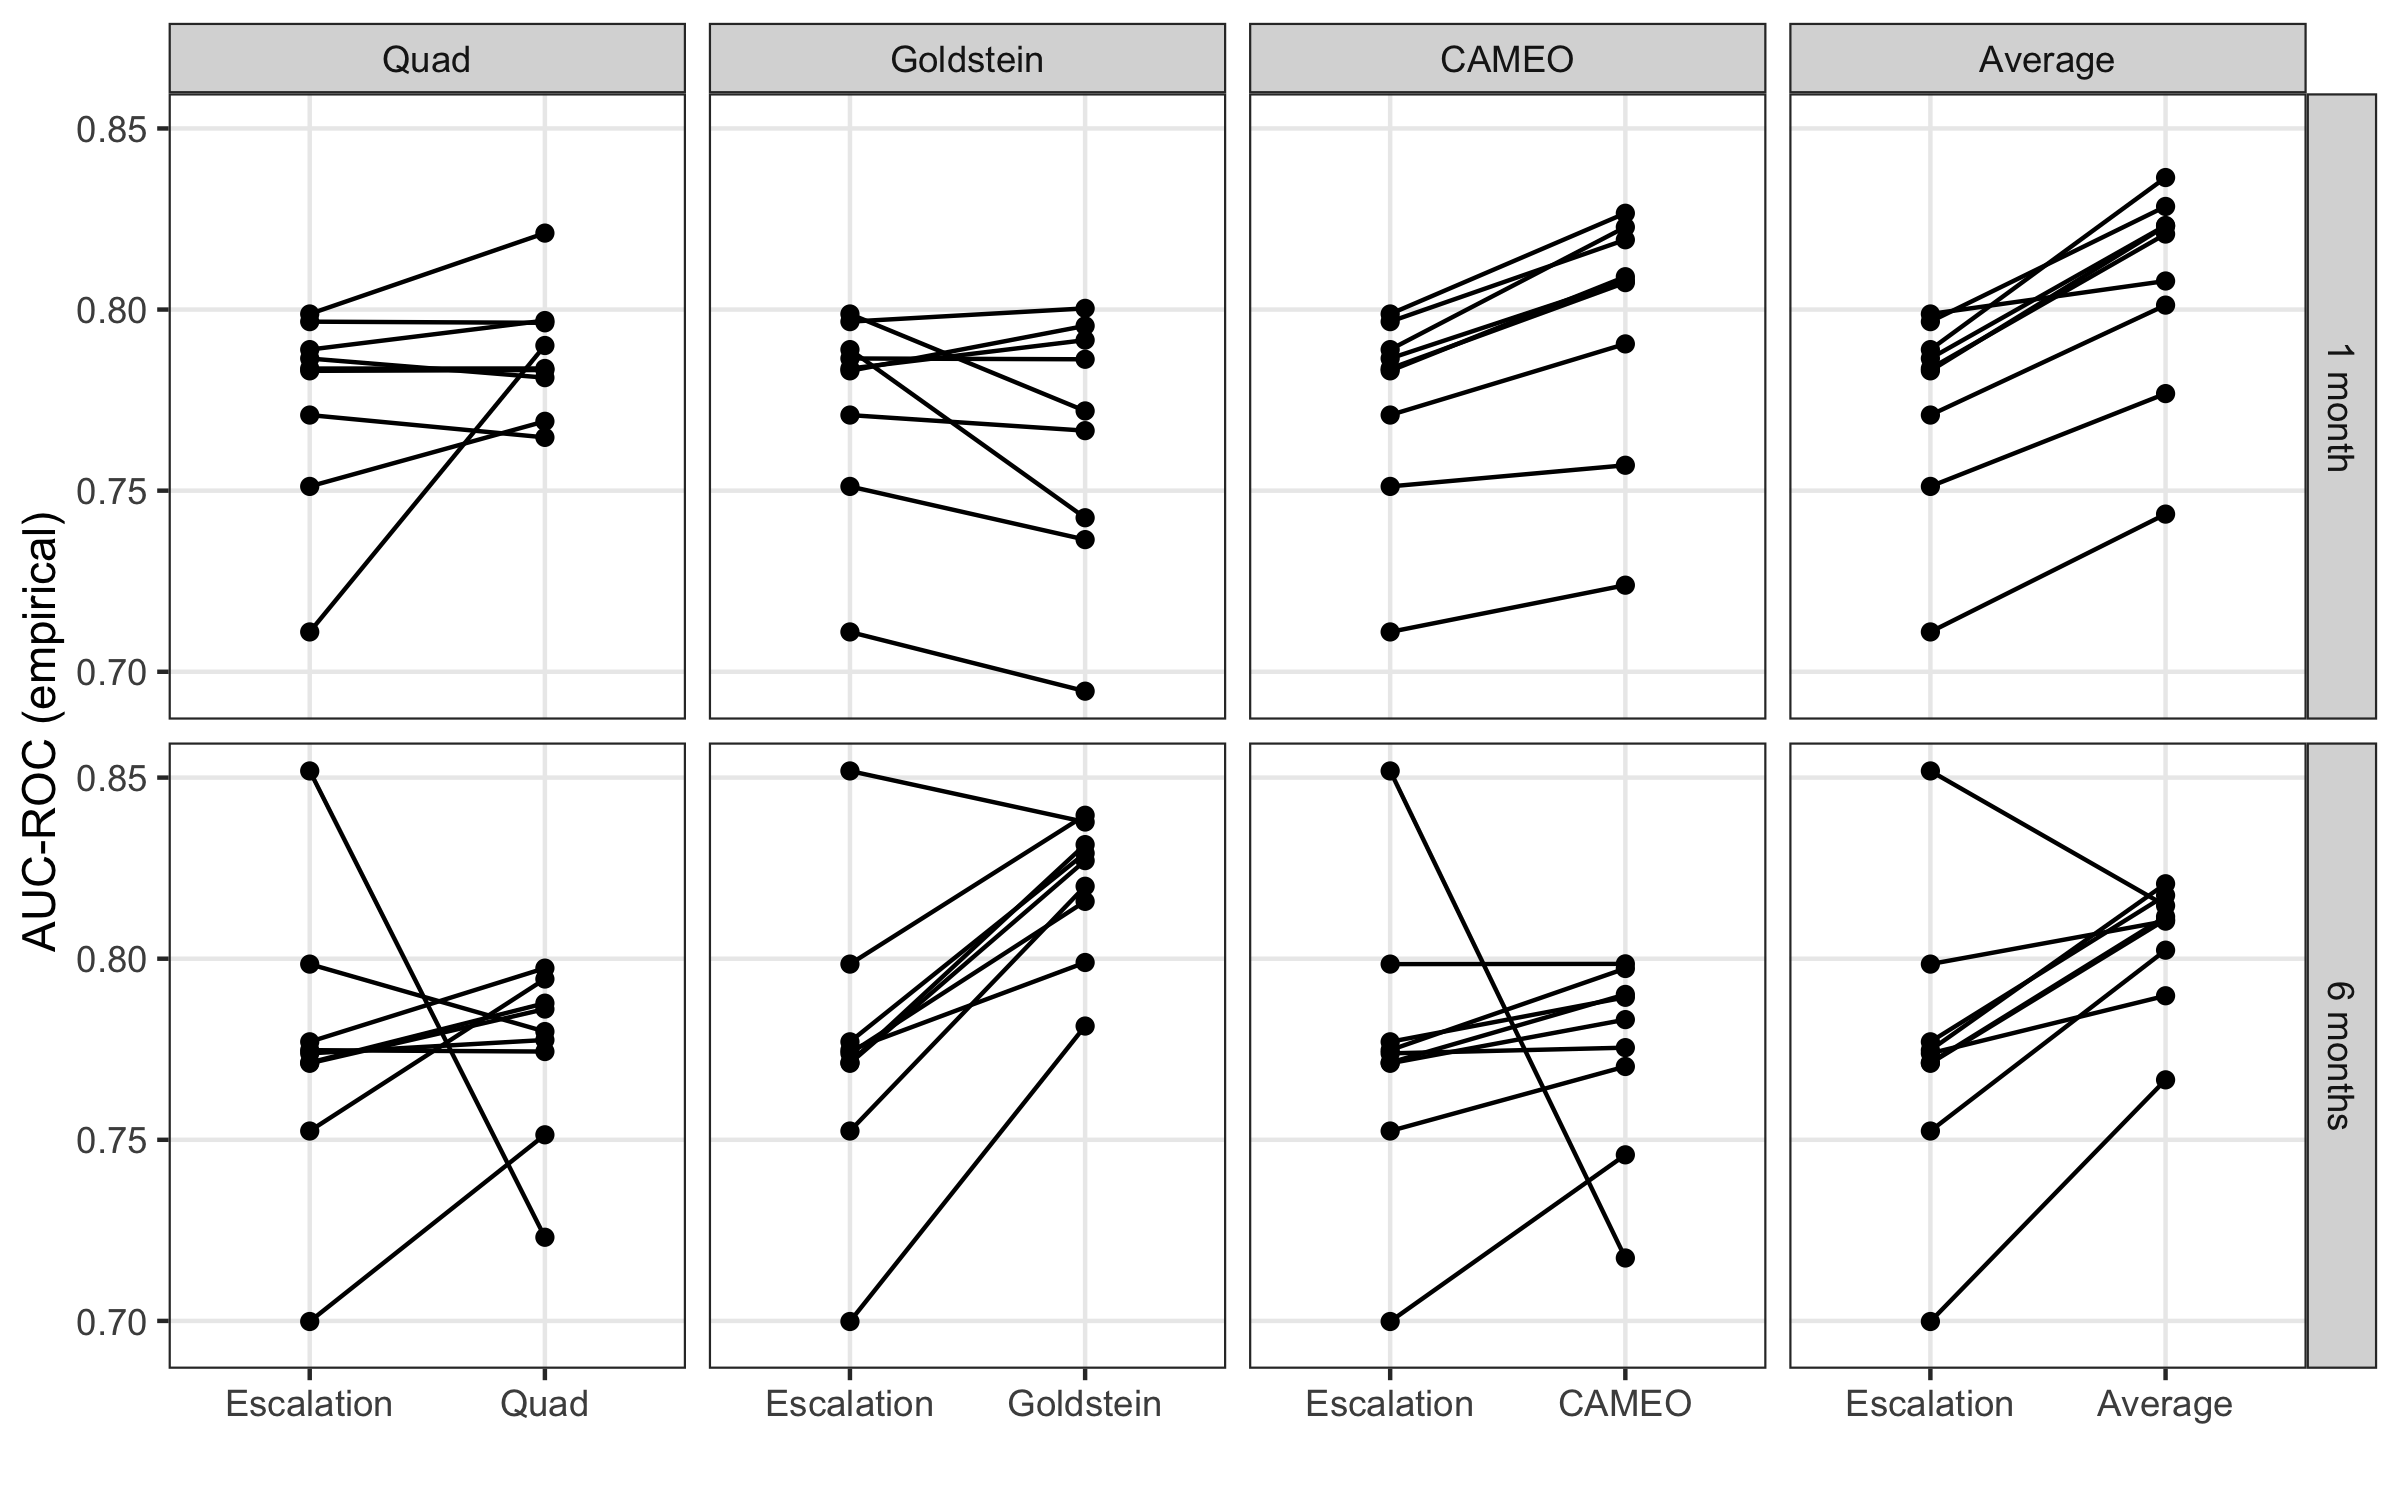
\includegraphics[width=.9\linewidth]{figures/fig-A1-table1-pairs.png}
}
\caption{Escalation to alternative comparisons for the ICEWS models (B\&S Table 1)\label{fig:table1-plot}}
\end{figure}

\begin{figure}
{\centering
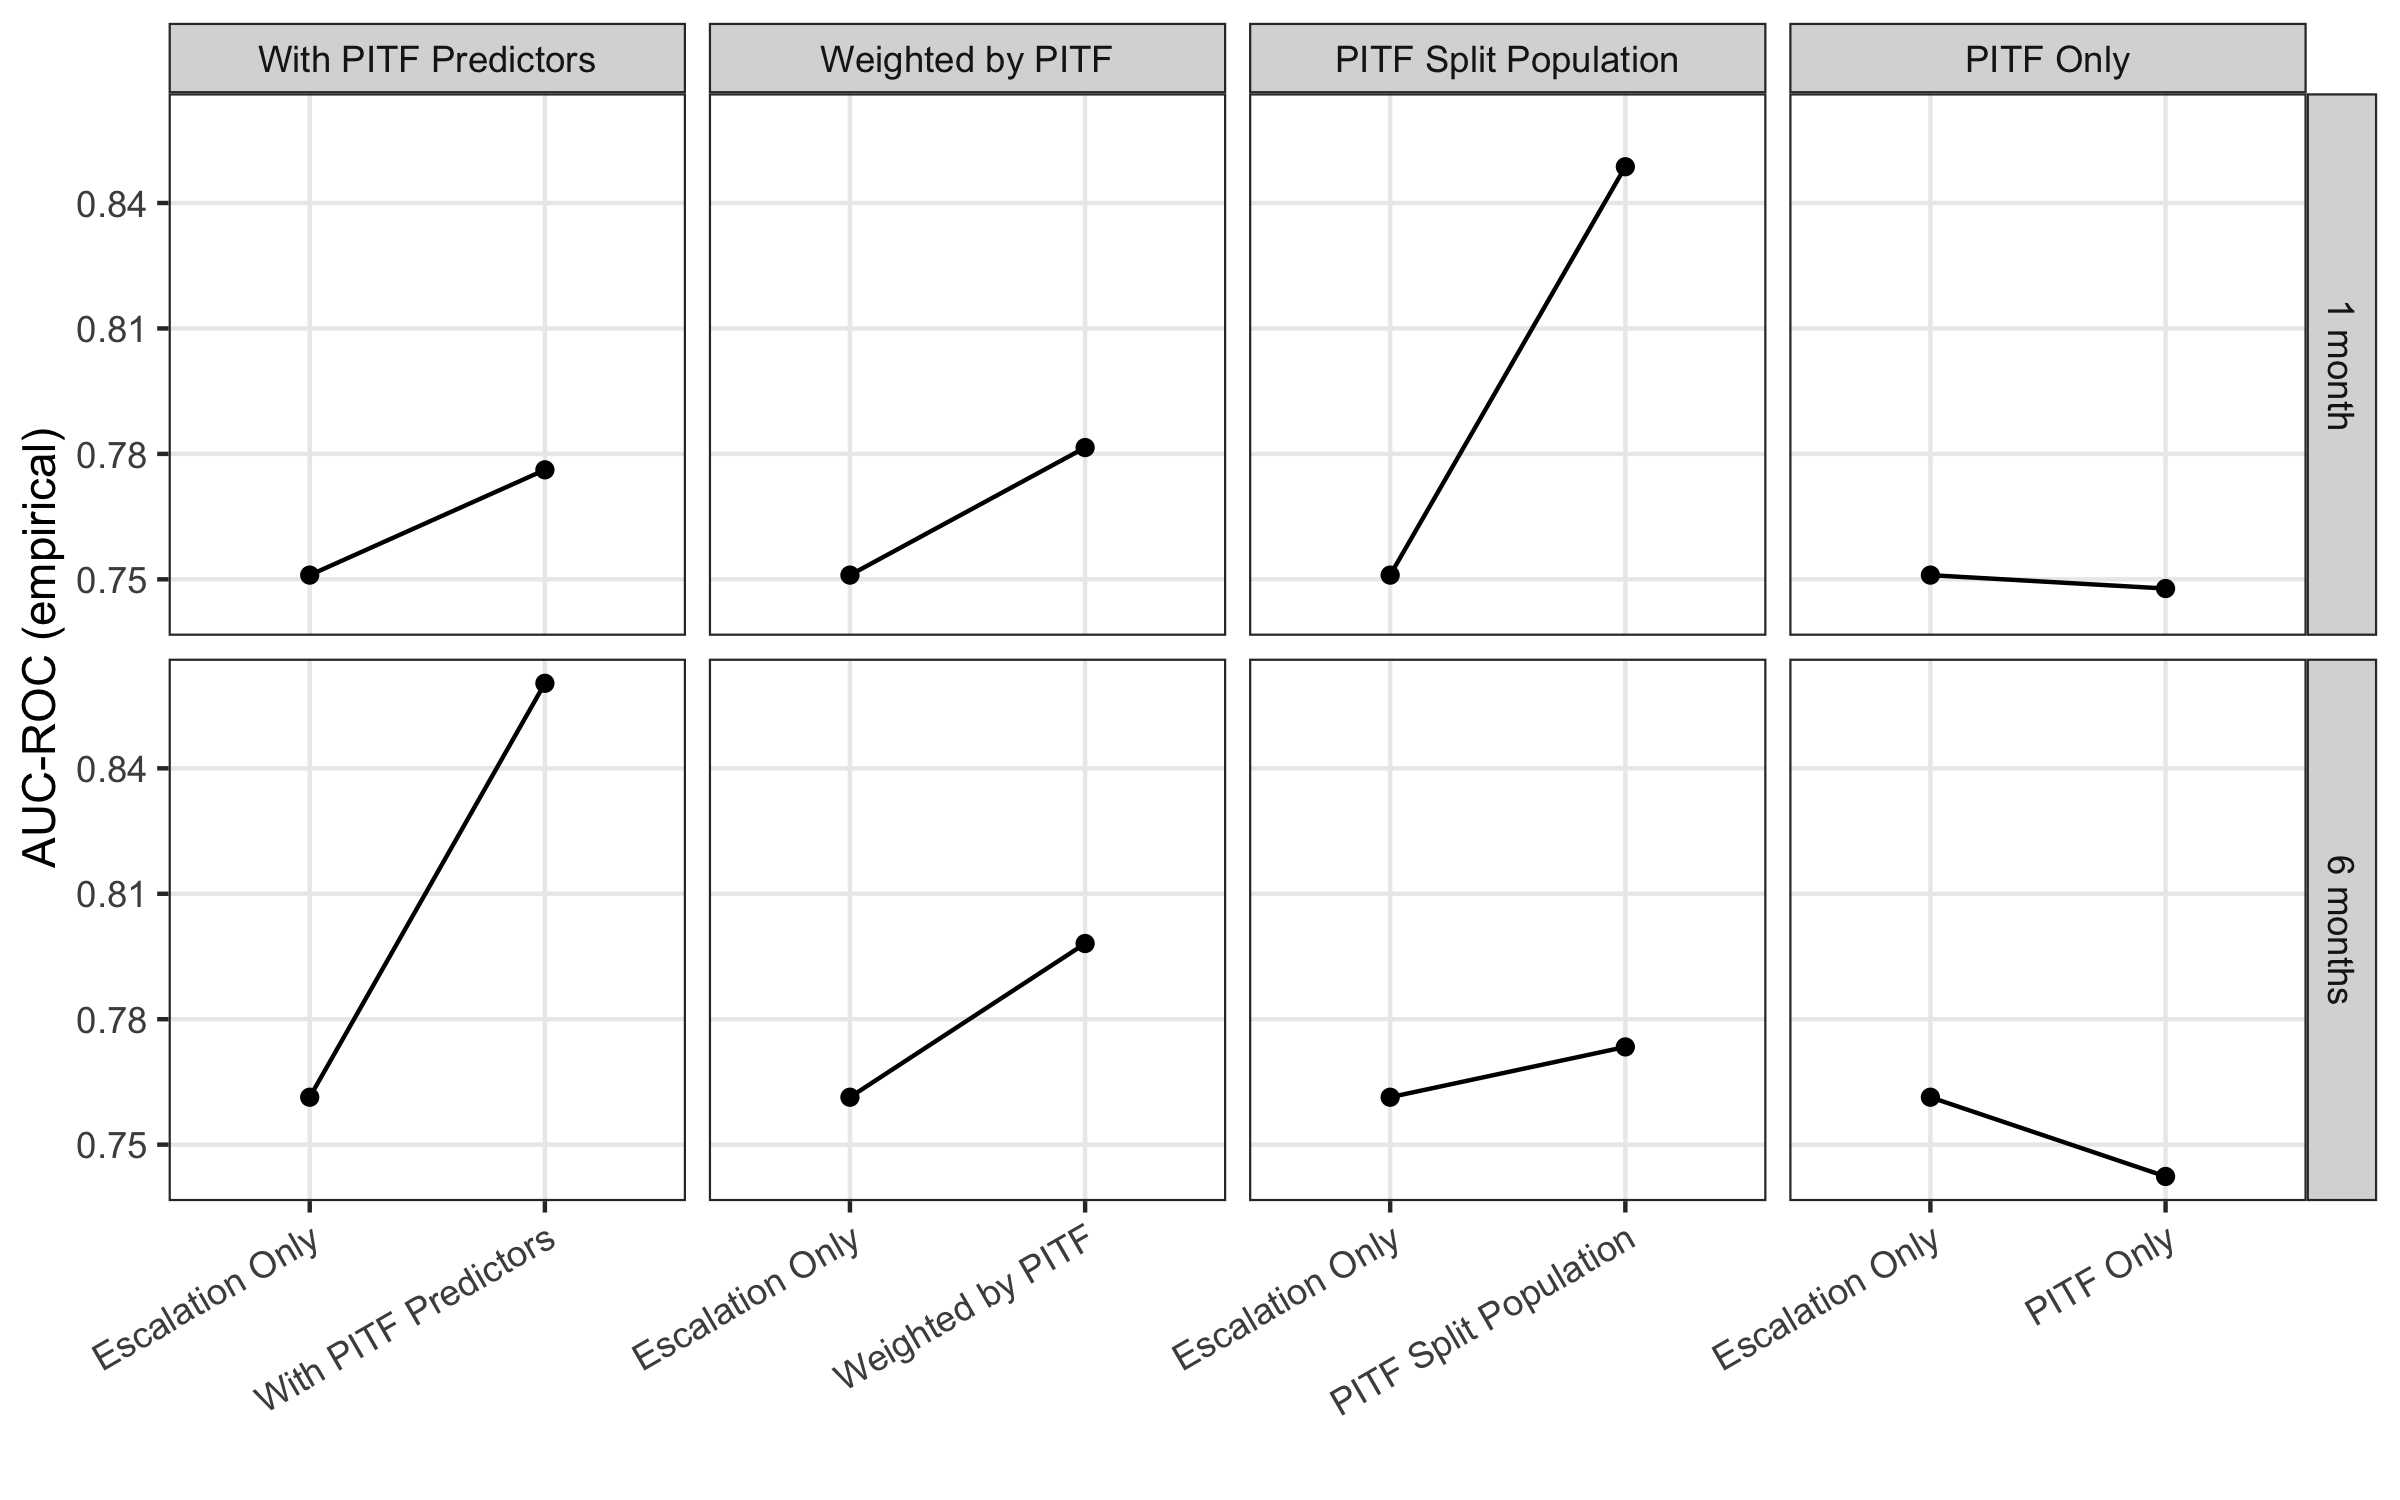
\includegraphics[width=.9\linewidth]{figures/fig-A2-table2-pairs.png}
}
\caption{Escalation to alternative comparisons for the structural models (B\&S Table 2)\label{fig:table2-plot}}
\end{figure}

\newpage

\hypertarget{random-forest-hyper-parameter-selection}{%
\subsection{Random forest hyper-parameter selection}\label{random-forest-hyper-parameter-selection}}

What initially sparked our interest in the paper was the unusual choice of hyperparameter settings for the random forest models estimated. Table \ref{tab:hp} shows the default values used by the implementation of random forest that B\&S use (from the \textbf{randomForest} R package), in contrast to the basic settings used by B\&S for most of the models reported in the paper.

As the outcome is a binary indicator of civil war onset, one would typically use a classification random forest that predicts 0 or 1 labels directly. The implementation of random forests that B\&S use ((Liaw and Wiener 2002)) is based on the original Breiman (2001) implementation and calculates predictive probabilities by averaging over the ``0'' or ``1'' votes from all constituent decision trees. The conventional wisdom regarding the number of trees in a random forest is that it needs to be large enough to stabilize performance, but without any additional gain or harm in accuracy beyond a certain number. From the other default settings, which are generally not uninformed choices, one can see that the basic logic is to grow a forest with a relatively small number of trees, but where each tree is fairly extensive and operates on a large bootstrapped sample of the original training data. These are of course only heuristics and it is usual to attempt to find better hyper-parameter methods through some form of tuning.

\begin{table}
\caption{\label{tab:hp} Random forest (\texttt{randomForest()}) default versus B\&S hyperparameters}
\begin{tabular}{l>{\raggedright\arraybackslash}p{2in}ll}
\toprule
Hyperparameter & Default heuristic & Default values (Escalation) & B\&S value \\
\midrule
type & & classification & regression \\
ntree & & 500 & 100,000 or 1e6 \\
mtry & \texttt{floor(sqrt(ncol(x)))} & 3 & 3 \\
replace & & true & false \\
sampsize & \texttt{nrow(x)} if replace, else \texttt{ceiling(.632*nrow(x))} & 11,869 & 100 or
500 \\
nodesize & 1 for classification & 1 & 1 \\
maxnodes & & null & 5 or 10 \\
\bottomrule
\end{tabular}
\end{table}

B\&S in contrast fit very large forests with 100,000 trees in the basic model form, but where each tree only operates on a very small sub-sample (N=100 or 500), drawn without replacement, of the available training data. This approach only works due to the choice to use regression, not classification, trees. Trying to use classification trees with the other parameter settings does not work at all because it is almost guaranteed that a sample of 100 from the \textasciitilde11,000 training data rows with 9 positive cases will only include 0 (negative) outcomes in the sample. As it is, using regression with a 0 or 1 outcome produces warnings when estimating the models:

\begin{verbatim}
Warning message:
In randomForest.default(y = as.integer(train_df$incidence_civil_ns_plus1 ==  :
  The response has five or fewer unique values.  Are you sure you want to do regression?
\end{verbatim}

As it turns out, using regression random forests for this kind of binary classification problem in order to obtain probability estimates matches the probability random forest approach suggested and positively evaluated in Malley et al. (2012), and which is used in another prominent R implementation of random forests.\footnote{The \textbf{ranger} package.} It is not clear whether this is intentional, as the Malley paper is not cited in B\&S.

In any case, B\&S's random forest approach appears to work really well. We tried to construct classification random forests tuned via cross-validation on the training data set partition, i.e.~without touching the test data, but were unable to develop models that consistently match the B\&S random forest method in both cross-validated out-of-sample training predictions and test set predictions.

Given that they are relatively unorthodox, yet appear to work very well, we wonder how the hyper-parameter values were determined. Two specific concerns are that this was not done with an eye towards test set accuracy, which would invalidate the independence of the out-of-sample test set, and whether the specific hyper-parameter values are optimized for only one model, or were optimized and found to work well for all models. There is no discussion of the random forest tuning strategy or how the specific hyper-parameter methods were determined in the paper.

Given the dramatic changes in results as a result of the preceding issues, we did not further investigate these potential concerns.

\newpage

\hypertarget{different-smoothing-methods}{%
\subsection{Different smoothing methods}\label{different-smoothing-methods}}

The \textbf{pROC} package \texttt{smooth()} function includes several different smoothing methods. The default, which BS use in their code, is binormal smoothing. Here is a replication of the smooth benefits shown in Figure \ref{fig:benefit-plot} with two other smoothing methods. (We could not get ``logcondens'' and ``logcondens.smooth'' to work, and they are based on another external package that has not been updated since 2016.)

Only the ``binormal'' smoothing method produces a pattern of AUC-ROCs that clearly elevates the Escalation model above the alternatives. The ``density'' method does not on average change the AUC-ROC values very much from their empirical ROC curve equivalents. The ``fitdistr'' method tends to increase all AUC-ROC values, although maybe slightly more so for the Escalation model than the main alternatives.

\begin{figure}
{\centering \includegraphics[width=.95\linewidth]{figures/fig-a3-benefit-plot-extended.png}}
\caption{Gain from using smoothed ROC to calculate AUC, for each model reported in Tables 3 and 4 (B\&S Tables 1 and 2), with 3 different smoothing methods (binormal is the default method and used in B\&S)\label{fig:smooth-benefit-plot-extended}}
\end{figure}

\end{document}
